\chapter{Robustness of codon models to mutational bias.}
\minitoc
\section{Abstract}

Protein-coding sequences subjected to mutational bias at the nucleotide level, and evolving under selection at the amino-acids will lean toward lower mutational bias when observed at the protein level. Unfortunately, parametric codon models developed to estimate the rate of evolution on amino-acids use the observed mutational bias at the protein level and don't take into account this effect. Thus, such parametric codon models are inherently misspecified to untangle mutation and selection, and they don't estimate the mutational process reliably. We also show that even if the mutational process is misspecified, parametric codon models are able to estimate reliably the rate of evolution acting on amino-acids. But if one wants to also estimate the mutational process, one need to use model where the rate of evolution is a tensor (95 parameters) instead of a single parameter.

\section{Notations}

\begin{itemize}
	\item $\Ne \in \mathbb{N}$ is the effective population size.
	\item $t \in \mathbb{R}_{\geq 0}$ is the time measured in unit of population size ($t=1 \Rightarrow 4 \Ne $ generations).
\end{itemize}

\subsection{\acrshort{DNA}}
\begin{itemize}
	\item $\mu \in \mathbb{R}_{\geq 0}$ is the \acrshort{DNA} mutation rate for one site of the sequence in one generation.
	\item $\theta=4 \Ne \mu \in \mathbb{R}_{>0} $ is the scaled mutation rate.
	\item $ \SetWeak = \left\{ A,T \right\} $ is the set of $2$ weak nucleotides ($2$ hydrogen bonds).
	\item $ \SetStrong = \left\{C,G \right\} $ is the set of $2$ strong nucleotides ($3$ hydrogen bonds).
	\item $\lambda \in \mathbb{R}_{\geq 0} $ is the relative rate of weak over strong mutations.
	\item $ \SetNuc = \SetWeak \cup \SetStrong =\left\{ A,C,G,T \right\} $ is the set of $4$ nucleotides in lexicographic order.
	\item $a \in \SetNuc $ and $b \in \SetNuc $ are used to denote nucleotides.
	\item $u_{a,b} \in \mathbb{R}_{> 0}$ is the mutation rate from nucleotide $a$ to $b$.
	\item $\bm{u} \in \mathbb{R}_{> 0}^{4 \times 4} $ is the mutation rate matrix between nucleotides.
	\item $\pi_a \in \left]0,1\right[ $ is the stationary distribution of nucleotide $a$. $\sum_{a \in \Omega_{\mathrm{Nuc}}} \pi_a = 1$.
	\item $\pi = \left(\pi_A , \pi_C , \pi_G , \pi_T \right) \in \left]0,1\right[^4$ is the vector of nucleotides stationary distribution.
\end{itemize}

\subsection{Codons}
\begin{itemize}
	\item $\SetCodon = \left\{ AAA,AAC, \dots, TTT \right\} $ is the set of $61$ non-stop codons in lexicographic order.
	\\By definition $\SetCodon = \left\{ \SetNuc \times \SetNuc \times \SetNuc \right\} \setminus \left\{ TAA, TAG, TGA \right\} $.
	\item $x \in \SetCodon $, $y \in \SetCodon $ and $y \in \SetCodon $ are used to denote the codons.
	\item $\NxAB \subset \SetCodon $ is the set of neighboring codons to codon $x$ such that the mutation is from nucleotide in $A \in \left\{ \SetWeak, \SetStrong \right\}$ to nucleotide in $B \in \left\{ \SetWeak, \SetStrong \right\}$.
	\item $\Nx =  \NxSS \cup \NxSW \cup \NxWS \cup \NxWW \subset \SetCodon $ is the set of neighboring codons to codon $x$.
	\item $w_x \in \left\{0,1,2,3 \right\}$ is the number of weak bases ($A$ and $T$) of codon $x$.
	\\For example $x=ACT \Rightarrow w_x=2$, or  $x=ACA \Rightarrow w_x=2$, or $x=ACG \Rightarrow w_x=1$.
	\item $U_{x,y} \in \mathbb{R}_{\geq 0} $ is the mutation rate from codon $x$ to $y$.
	\item $n \in \mathbb{N}$ is the number of codon sites in the sequence.
	\item $k \in \left\{ k \in \mathbb{N} \mid 1 \leq k \leq n \right\}$ is the $k^{\mathrm{th}}$ codon site of the sequence.
	\item $Q_{x,y}^{(k)} \in \mathbb{R}_{\geq 0} $ is the substitution rate from codon $x$ to $y$ at site $k$.
	\item $\bm{Q}^{(k)} \in \mathbb{R}_{\geq 0}^{61 \times 61} $ is the substitution rate matrix of codons at site $k$.
	\item $\Pi_x^{(k)} \in \left]0,1\right[ $ is the stationary distribution of codon $x$ at site $k$. $\sum_{x \in \SetCodon} \Pi_x^{(k)} = 1$.
	\item $\Pi^{(k)} = \left( \Pi_x , \ \forall x \in \SetCodon \right) \in \left]0,1\right[^{61} $ is the vector of codon stationary distribution.
\end{itemize}

\subsection{Amino-acids}
\begin{itemize}
	\item $\SetAa = \left\{ \mathrm{Arginine}, \dots ,\mathrm{Tyrosine} \right\} $ is the set of 20 amino-acids in lexicographic order.
	\item $X \in \SetAa $, $Y \in \SetAa$ and $Y \in \SetAa$ are used to denote the amino-acid encoded by codon $x$ and $y$.
	\\For example $x=ACT \Rightarrow X=$ Threonine.
	\item $\NxNonSyn \subset \Nx $ is the set of non-synonymous neighboring codons of codon $x$.
	\\By definition $\NxNonSyn = \left\{ y \in \Nx  \mid \ Y \neq X  \right\} $.
	\item $\NxSyn \subset \Nx $ is the set of synonymous neighboring codons of codon $x$.
	\\By definition $\NxSyn = \left\{ y \in \Nx \mid \ Y = X  \right\} $ and $\NxSyn \cup \NxNonSyn = \Nx $.
	\item $F_X^{(k)} \in \mathbb{R} $ is the fitness of amino-acid $X$, and thus of codon $x$ at site $k$.\\
	The fitness are normalized such that $\sum_{X \in \SetAa}\e^{F_X^{(k)}} = 1 $
	\item $F^{(k)} = \left( F_X , \ \forall X \in \SetAa \right) \in \mathbb{R}^{20} $ is the vector of amino-acids fitness at site $k$.
	\item $\bm{F} = \left( F^{(k)} , \  1 \leq k \leq n \right) \in \mathbb{R}^{20 \times n} $ is the matrix of amino-acids fitness for the whole sequence.
\end{itemize}

\subsection{Distribution of fitness effects}
\begin{itemize}
	\item $s_X = \e^{F_X} \in \left]0,1\right[ $ is the propensity of amino-acid $X$.\\
	The propensities are normalized such that $\sum_{X \in \SetAa}s_X = 1 $.
	\item $s = \left( s_X , \forall X \in \SetAa \right) \in \left]0,1\right[^{20} $ is the vector of amino-acids propensities.
	\item $C(s) = \left\{ s \mid \sum_{X \in \SetAa} s_X = 1  \right\} $ is the $19$-dimensional simplex of propensities.
	\item $\forall z \in \mathbb{R}_{>0}, \ \Gamma(z) = \int_{0}^{\infty} x^{z-1} \e^{-x} \der x \in \mathbb{R}_{>0} $ is the gamma function.
	\item $\mathrm{Dirichlet}(\alpha, 20)$ is the Dirichlet distribution of order $20$ with concentration parameter $\alpha \in \mathbb{R}_{>0}$.
	\item $p(z) \in \mathbb{R}_{\geq 0}$ is the probability density function of the continuous random variable $Z$.
	\item $S \sim \mathrm{Dirichlet}(\alpha, 20) \Rightarrow	p(s; \alpha) = {\frac {\Gamma (20 \alpha)}{\Gamma (\alpha )^{20}}} \prod_{X \in \SetAa} s_X^{\alpha-1}, \ \forall s \in C(s)$.
	\item $\operatorname{E}[f(S)] = \int_{C(s)} f(s) p(s; \alpha) \der s$ is the expected value of $f(S)$ for any function $f$.
\end{itemize}

\section{Summary}

The nucleotide frequencies in protein-coding sequences is the result of the equilibrium between mutation and
selection. As a consequence, protein-coding sequences subjected to mutational bias at the nucleotide level,
and evolving under selection at the amino-acids, will lean toward lower mutational bias when observed at
the protein level. Unfortunately, parametric codon models developed to estimate the rate of evolution on
amino-acids use the observed mutational bias at the protein level and don’t take into account this effect.
Thus, such parametric codon models are inherently misspecified to untangle mutation and selection, and
they don’t estimate the mutational process reliably. We also show that even if the mutational process is
misspecified, parametric codon models are able to estimate reliably the rate of evolution acting on amino-
acids. But if one wants to also estimate the mutational process, one need to use model where the rate of
evolution is a tensor (95 parameters) instead of a single parameter.
We seek to simulate the evolution of protein-coding sequences along a specie tree. Starting with one
sequence at the root of the tree, the sequences evolves independently along the different branches of the
tree, until they reach the leaves. At the end of the simulation, we get one sequence for each leaf of the
tree, meaning one sequence per specie. Such evolutionary process is an idealized version of the reality, in
the sens that the whole heterogeneity of sequences in the population is wiped away, with only one sequence
representing the whole population. To make such idealized process more realistic, one can use population-
genetic framework. In population-genetics, a change in the whole population sequence, called substitution,
is modeled as the product of a mutation and a fixation. A mutation only appear in one specific individual of
the population, and a fixation is the probability that this specific individual is eventually a parent of all the
population later in time. One interesting result of population genetic is that the substitution rate is equal to
the mutation rate if the mutations are selectively neutral. If a mutation is favored (disfavored) by selection,
the substitution rate is higher (lower) than the neutral rate.
For a protein-coding \acrshort{DNA} sequence, a substitution is modeled as the product of mutation at the nucleotide
level, and selection of the amino-acid level. On one hand, the mutation rate between nucleotides as assumed
to be same for all sites of the sequences. On the other hand, the selection for amino-acids is not assumed
to be the same for all sites of the sequences. For example, an exterior site (solvent accessible residue) might
favor hydrophilic amino-acids, and an interior site of the protein might favor hydrophobic amino-acids.


\section{Introduction}

We seek to simulate the evolution of protein-coding sequences along a specie tree.
Starting with one sequence at the root of the tree, the sequences evolves independently along the different branches of the tree, until they reach the leaves. At the end of the simulation, we get one sequence for each leaf of the tree, meaning one sequence per specie.
Such evolutionary process is an idealized version of the reality, in the sens that the whole heterogeneity of sequences in the population is wiped away, with only one sequence representing the whole population. To make such idealized process more realistic, one can use population-genetic framework. In population-genetics, a change in the whole population sequence, called substitution, is modeled as the product of a mutation and a fixation. A mutation only appear in one specific individual of the population, and a fixation is the probability that this specific individual is eventually a parent of all the population later in time. One interesting result of population genetic is that the substitution rate is equal to the mutation rate if the mutations are selectively neutral. If a mutation is favored (disfavored) by selection, the substitution rate is higher (lower) than the neutral rate.\\

For a protein-coding DNA sequence, a substitution is modeled as the product of mutation at the nucleotide level, and selection of the amino-acid level. On one hand, the mutation rate between nucleotides as assumed to be same for all sites of the sequences. On the other hand, the selection for amino-acids is not assumed to be the same for all sites of the sequences. For example, an exterior site (solvent accessible residue) might favor hydrophilic amino-acids, and an interior site of the protein might favor hydrophobic amino-acids.

\section{Simulation of protein-coding sequences evolution}

\subsection{Modeling mutational bias}
\label{sec:mutBias}
The mutation rate between nucleotides is always proportional to $\mu$. Moreover, mutations from any nucleotide to another weak nucleotide is increased by the factor $\lambda$ compared with mutations to another strong nucleotides. The rate at which a nucleotide doesn't change is given such the sum of all rates is zero.
\begin{equation}
\label{nucRates}
u_{a, b} =
\begin{dcases}
\mu
& \mathrm{if} \ b \in \SetStrong \ \mathrm{ and } \ a \neq b, \\
\mu \lambda
& \mathrm{if} \ b \in  \SetWeak \ \mathrm{ and } \ a \neq b,  \\
- \sum_{b \in \SetNuc, \ b \neq a }  u_{a, b}
& \mathrm{if} \ a = b.
\end{dcases}
\end{equation}
And the matrix of mutation rates is:
\begin{equation}
\label{nucMatrix}
\bm{u} =
\begin{pmatrix}
{-\mu(2 + \lambda)} & {\mu} & {\mu} & {\mu \lambda} \\
{\mu \lambda} & {-\mu(1 + 2\lambda)} & {\mu} & {\mu \lambda} \\
{\mu \lambda} & {\mu} & {-\mu(1 + 2\lambda)} & {\mu \lambda} \\
{\mu \lambda} & {\mu} & {\mu} & {-\mu(2 + \lambda)}
\end{pmatrix}.
\end{equation}
The stationary distribution $\Pi$ must be annihilated by the mutation matrix $\bm{u}$, which gives the stationary distribution:
\begin{align}
\pi \bm{u}
& =0, \\
\iff \pi
& =\left( \dfrac{\lambda}{2+2\lambda}, \dfrac{1}{2+2\lambda}, \dfrac{1}{2+2\lambda}, \dfrac{\lambda}{2+2\lambda} \right), \\
\iff \pi_a
& = &
\begin{dcases}
\dfrac{1}{2+2\lambda} & \mathrm{if} \ a \in \SetStrong, \\
\dfrac{\lambda}{2+2\lambda} & \mathrm{if} \ a \in  \SetWeak.  \\
\end{dcases}
\label{nucStationarity}
\end{align}
The process is reversible and fulfills detailed balance conditions for any pair of different nucleotides:
\begin{align}
\pi_a u_{a, b}
& = &
\begin{cases}
( 2 + 2 \lambda)^{-1} \mu
& \mathrm{if} \ a \in \SetStrong, \ b \in \SetStrong \ \mathrm{ and } \ a \neq b,\\
( 2 + 2 \lambda)^{-1} \mu \lambda
& \mathrm{if} \ a \in \SetStrong, \ b \in \SetWeak \ \mathrm{ and } \ a \neq b, \\
\lambda  ( 2 + 2 \lambda)^{-1} \mu
& \mathrm{if} \ a \in \SetWeak, \ b \in \SetStrong \ \mathrm{ and } \ a \neq b,\\
\lambda ( 2 + 2 \lambda)^{-1} \mu \lambda
& \mathrm{if} \ a \in \SetWeak, \ b \in \SetWeak \ \mathrm{ and } \ a \neq b, \ \textrm{from eq.}\ \ref{nucRates} \text{ and } \ \ref{nucStationarity},
\end{cases} \\
& =\pi_b u_{b, a} .
\label{nucMutBalance}
\end{align}
It is important to note that ratio of weak over strong nucleotides frequency at stationarity is equal to $\lambda$:
\begin{align}
\label{lambda}
\dfrac{ \pi_A + \pi_T }{ \pi_C + \pi_G }
& =\dfrac{ \lambda ( 2 + 2 \lambda)^{-1} + \lambda ( 2 + 2 \lambda)^{-1}}{ ( 2 + 2 \lambda)^{-1} +  ( 2 + 2 \lambda)^{-1}}, \ \textrm{from eq.}\ \ref{nucStationarity},\\
& =\lambda .
\end{align}

\subsection{Modeling selection at the amino-acid level}
The mutation rate between a pair of codons is given by the underlying mutation rates between nucleotides. However the rate mutation rate is null if the pair of codons differs by more than one nucleotide:
\begin{equation}
\label{codonMutRates}
U_{x, y} =
\begin{cases}
\mu
& \mathrm{if} \ y \in  \NxSS \cup \NxWS \ \mathrm{ and } \ x \neq y, \\
\mu \lambda
& \mathrm{if} \ y \in \NxSW \cup \NxWW   \ \mathrm{ and } \ x \neq y, \\
0
& \mathrm{if} \  y \notin \Nx \ \mathrm{ and } \ x \neq y, \\
- \sum_{y \in \Nx }  U_{x, y} & \mathrm{if} \ x = y.
\end{cases}
\end{equation}
To note, the substitution rate between codons would be equal to the mutation rate of \ref{codonMutRates} if codons are selectively neutral. However, we subsequently take into the selection acting on codon by modeling it at the amino-acid level, where each amino-acid ($X \in \SetAa$ are given a fitness ($F_X$). By modeling fitness at the amino-acid level, we assume that all codons encoding for one particular amino-acid are selectively neutral. In this modeling framework, the genetic code is of particular importance since the number of codons encoding for a particular amino-acid varies greatly. As an example, Tryptophan is encoded by one codon, while Leucine is encoded by 6 codons. Intuitively, this variation makes the mutation bias more effective in codons encoding for many amino-acids since there are many mutations possible that are selectively neutral (same amino-acid). While the other hand, the mutation bias is more constrained if the amino-acid is encoded by a few codons since there is only a few mutations possible that are selectively neutral.\\

To take into account the heterogeneity of selection between different sites of the protein, we assume that each site $k$ of the sequence is evolving under a different fitness landscape ($F_X^{(k)}, \ \forall X \in \SetAa $).
At one particular site, under a static fitness landscape, the substitution rate between codons are given by the product of the mutation rate and the probability of fixation, given by the formula of Kimura (1983) \citep{kimura_neutral_1983}:
\begin{equation}
\label{codonSubRates}
Q_{x, y}^{(k)} =
\begin{dcases}
U_{x, y}
& \mathrm{if} \ y \in \NxSyn \ (y \in \Nx \ \mathrm{and} \ X = Y),  \\
U_{x, y} \dfrac{F_Y^{(k)} - F_X^{(k)}}{1 - \e^{F_X^{(k)} - F_Y^{(k)}}}
& \mathrm{if} \ y \in \NxNonSyn \ (y \in \Nx \ \mathrm{and} \ X \neq Y),  \\
0
& \mathrm{if} \  y \notin \Nx \ \mathrm{ and } \ x \neq y, \\
- \sum_{y \in \Nx }  Q_{x, y}^{(k)}
& \mathrm{if} \ x = y.  \\
\end{dcases}
\end{equation}
The stationary distribution $\Pi$ must be annihilated by the mutation matrix $\bm{Q}$, which gives the stationary distribution at site $k$:
\begin{align}
\Pi^{(k)} \bm{Q}^{(k)}
& =0 ,\\
\iff \Pi_x^{(k)}
& =A^{(k)} \lambda^{w_x} \e^{F_X^{(k)}} ,\ \forall x \in \SetCodon,\\
& \mathrm{ where } \ A^{(k)} = \left( \sum_{y \in \SetCodon} \lambda^{w_y} \e^{F_Y^{(k)}} \right)^{-1}.
\label{codonStationarity}
\end{align}
Interestingly, the mutation process between codons fulfills an equation similar to detailed balance conditions:
\begin{align}
\lambda^{w_x} U_{x, y}
& = &
\begin{cases}
\lambda^{w_x} \mu
& \mathrm{if} \ y \in \NxSS, \\
\lambda^{w_x} \mu \lambda
& \mathrm{if} \ y \in \NxSW, \\
\lambda^{w_x} \mu
& \mathrm{if} \ y \in \NxWS, \\
\lambda^{w_x} \mu \lambda
& \mathrm{if} \ y \in \NxWW, \ \textrm{from eq.}\ \ref{nucRates},
\end{cases} \\
& = &
\begin{cases}
\lambda^{w_y} \mu
& \mathrm{if} \ y \in \NxSS, \\
\lambda^{w_y - 1} \mu \lambda
& \mathrm{if} \ y \in \NxSW, \\
\lambda^{w_y + 1} \mu
& \mathrm{if} \ y \in \NxWS, \\
\lambda^{w_y} \mu \lambda
& \mathrm{if} \ y \in \NxWW, \ \textrm{by definition of} \ w_x \ \text{and} \ w_y,
\end{cases} \\
& = &
\begin{cases}
\lambda^{w_y} \mu
& \mathrm{if} \ y \in \NxSS, \\
\lambda^{w_y} \mu
& \mathrm{if} \ y \in \NxSW, \\
\lambda^{w_y} \mu \lambda
& \mathrm{if} \ y \in \NxWS, \\
\lambda^{w_y} \mu \lambda
& \mathrm{if} \ y \in \NxWW, \ \textrm{by factoring} \ \lambda,
\end{cases} \\
& = &
\begin{cases}
\lambda^{w_y} \mu
& \mathrm{if} \ x \in \NySS, \\
\lambda^{w_y} \mu
& \mathrm{if} \ x \in \NyWS, \\
\lambda^{w_y} \mu \lambda
& \mathrm{if} \ x \in \NySW, \\
\lambda^{w_y} \mu \lambda
& \mathrm{if} \ x \in \NyWW, \ \textrm{since} \ x \in \NxAB \iff y \in \NyBA,
\end{cases} \\
& = &
\lambda^{w_y} U_{y,x}.
\label{codonMutBalance}
\end{align}
Moreover, the substitution process is reversible and fulfills detailed balance conditions at each site $k$:
\begin{align}
\Pi_x^{(k)} Q_{x, y}^{(k)}
& =A^{(k)} \lambda^{w_x} \e^{F_X^{(k)}}
\begin{cases}
U_{x, y}
& \mathrm{if} \ y \in \NxSyn,  \\
U_{x, y} \dfrac{F_Y^{(k)} - F_X^{(k)}}{1 - \e^{F_X^{(k)} - F_Y^{(k)}}}
& \mathrm{if}  \ y \in \NxNonSyn, \ \textrm{from eq.}\ \ref{codonSubRates} \text{ and } \ \ref{codonStationarity},
\end{cases} \\
& =A^{(k)} \lambda^{w_x} U_{x, y}
\begin{cases}
\e^{F_X^{(k)}}
& \mathrm{if} \ y \in \NxSyn,  \\
\dfrac{F_Y^{(k)} - F_X^{(k)}}{ \e^{-F_X^{(k)}}  - \e^{- F_Y^{(k)}} }
& \mathrm{if}  \ y \in \NxNonSyn, \ \textrm{by rearranging},
\end{cases} \\
& =A^{(k)} \lambda^{w_y} U_{y, x}
\begin{cases}
\e^{F_Y^{(k)}}
& \mathrm{if} \ y \in \NxSyn , \\
\e^{F_Y^{(k)}} \dfrac{F_Y^{(k)} - F_X^{(k)}}{ \e^{F_Y^{(k)}-F_X^{(k)}} - 1 }
& \mathrm{if}  \ y \in \NxNonSyn, \ \textrm{from eq.} \ \ref{codonMutBalance}
\end{cases} \\
& =A^{(k)} \lambda^{w_y} \e^{F_Y^{(k)}}
\begin{cases}
U_{y, x}
& \mathrm{if} \ x \in \NySyn, \ \textrm{since} \ y \in \NxSyn \iff x \in \NySyn,  \\
U_{y, x} \dfrac{F_X^{(k)} - F_Y^{(k)}}{1 - \e^{F_Y^{(k)}-F_X^{(k)}}}
& \mathrm{if}  \ x \in \NyNonSyn, \ \textrm{since} \ y \in \NxNonSyn \iff x \in \NyNonSyn,
\end{cases} \\
& =\Pi_y^{(k)} Q_{y, x}^{(k)} .
\label{codonSubBalance}
\end{align}

\begin{figure}[thbp]
	\begin{center}
		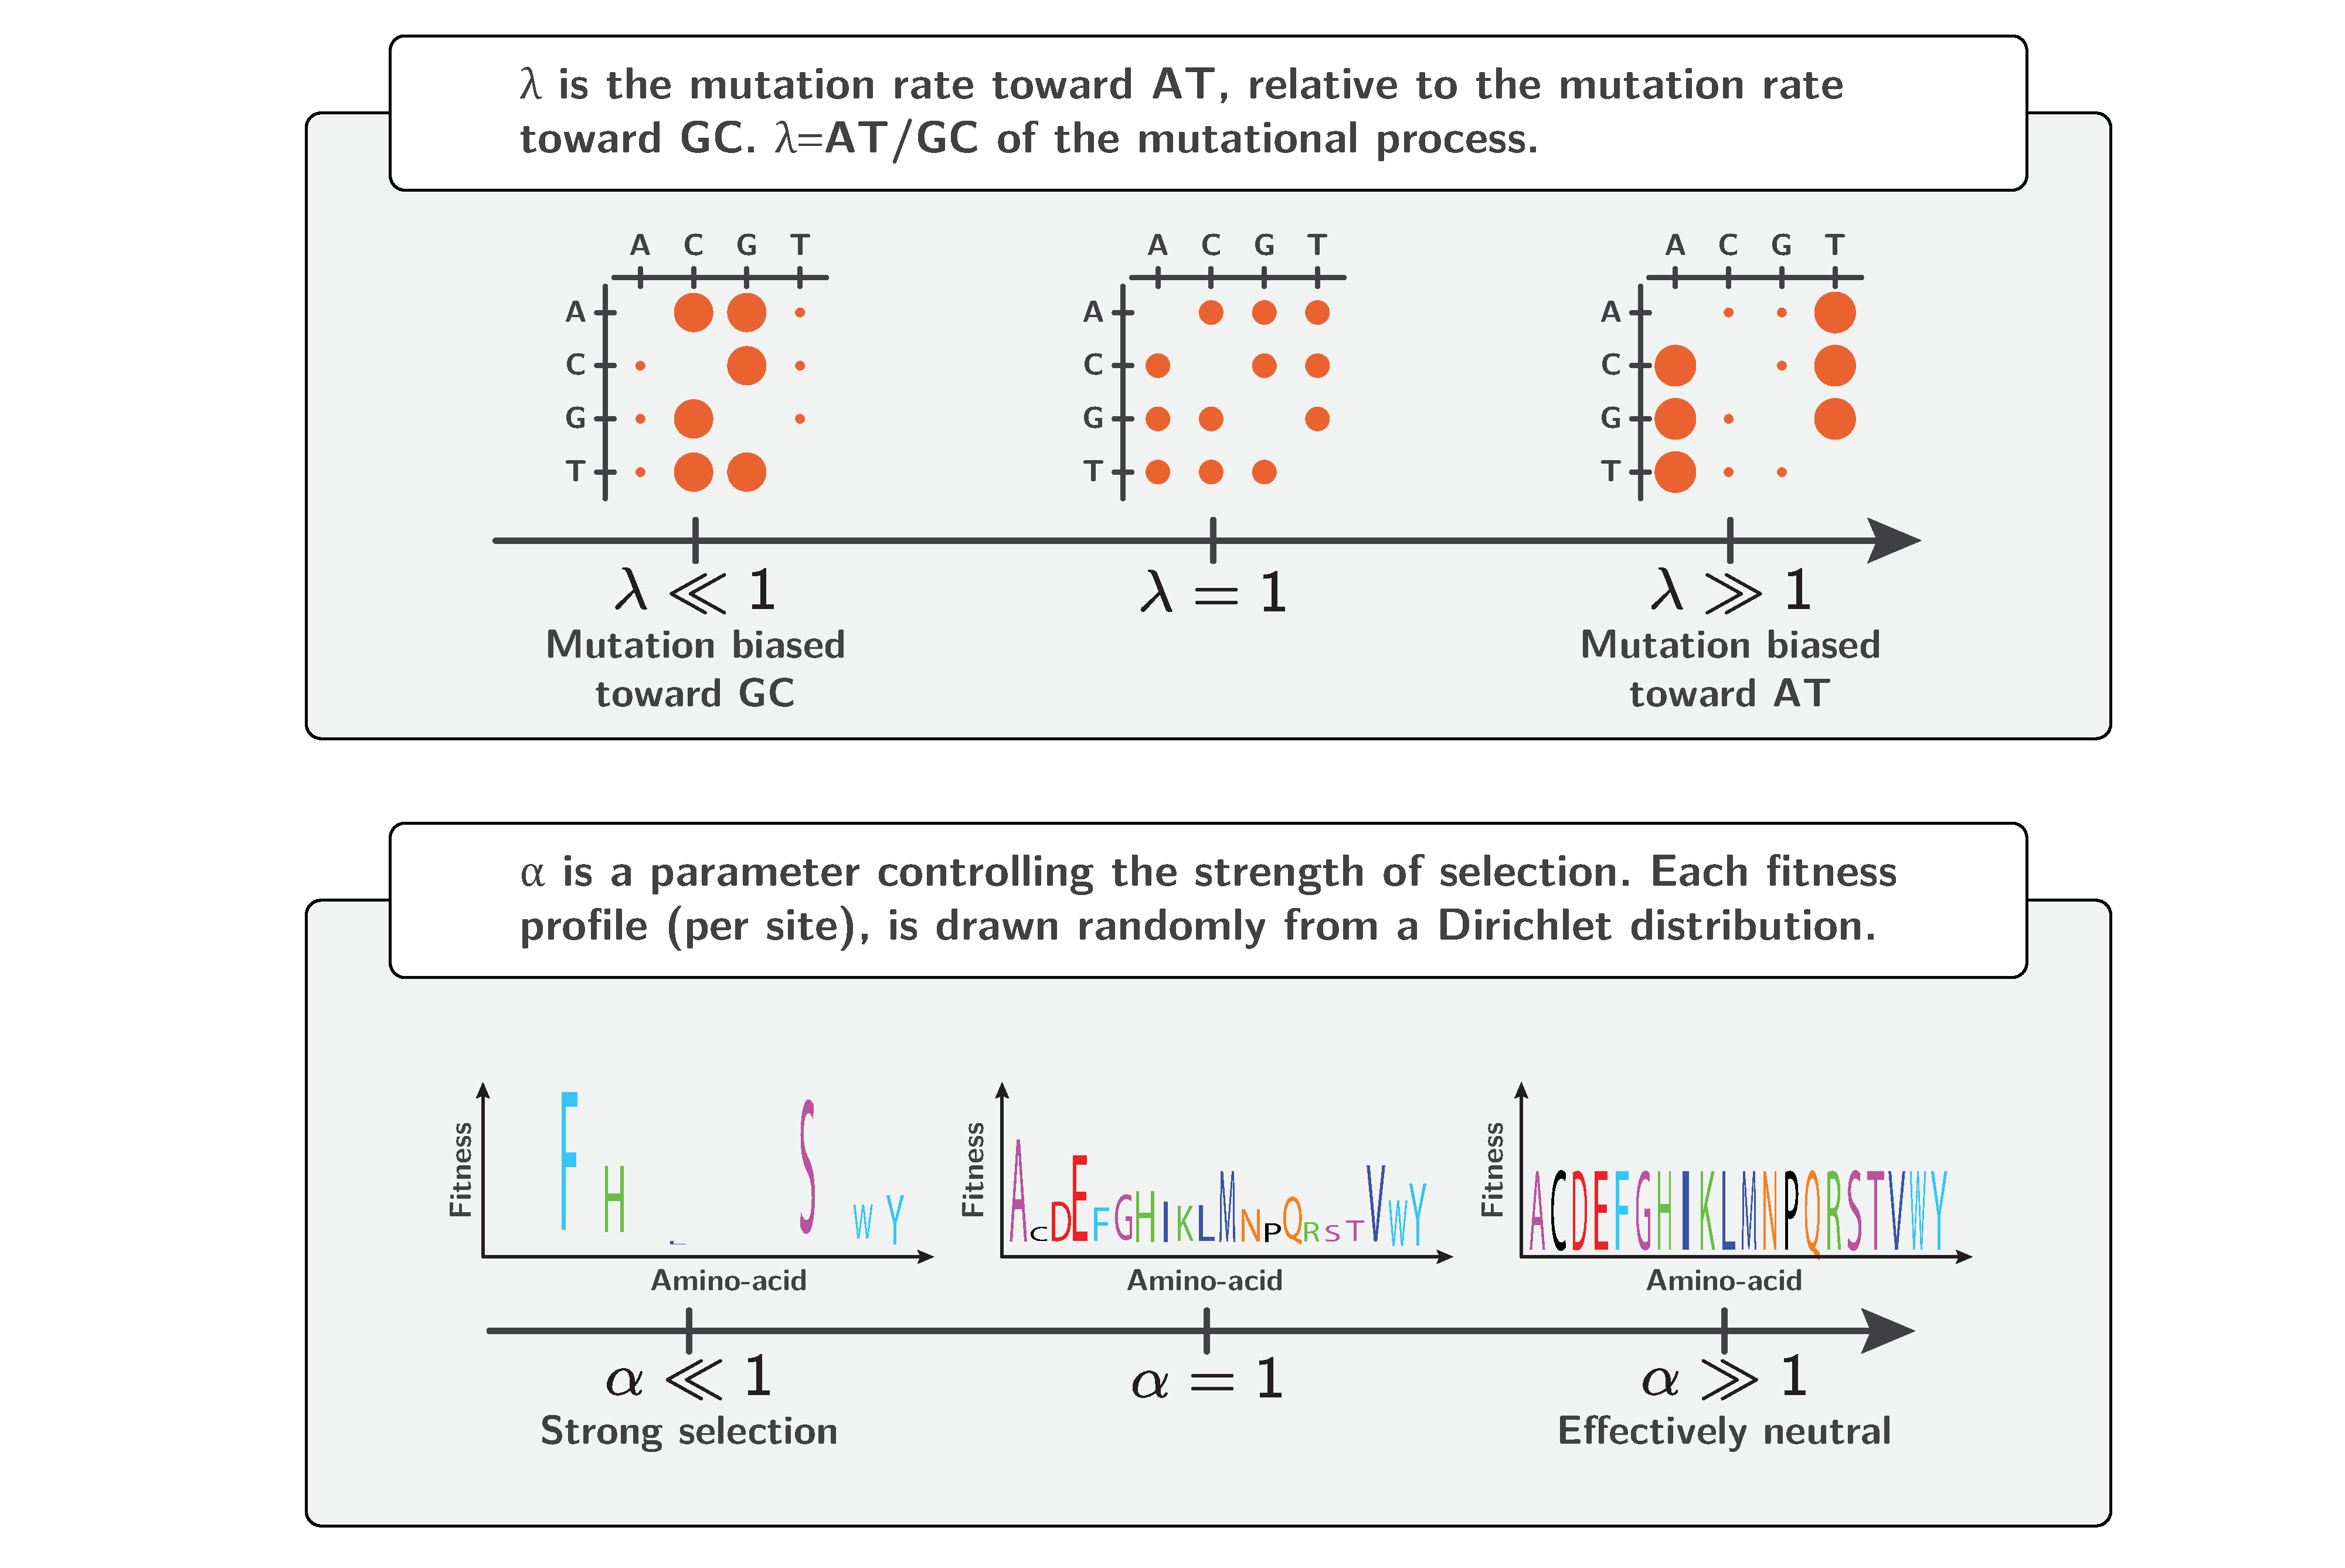
\includegraphics[width=\textwidth] {figures/mut-bias-parameters}
	\end{center}
	\caption[Parameters of the mutation-selection model]{Parameters of the mutation-selection model. One parameter for mutational bias, and one for strength of selection.}
\end{figure}

\begin{figure}[thbp]
	\begin{center}
		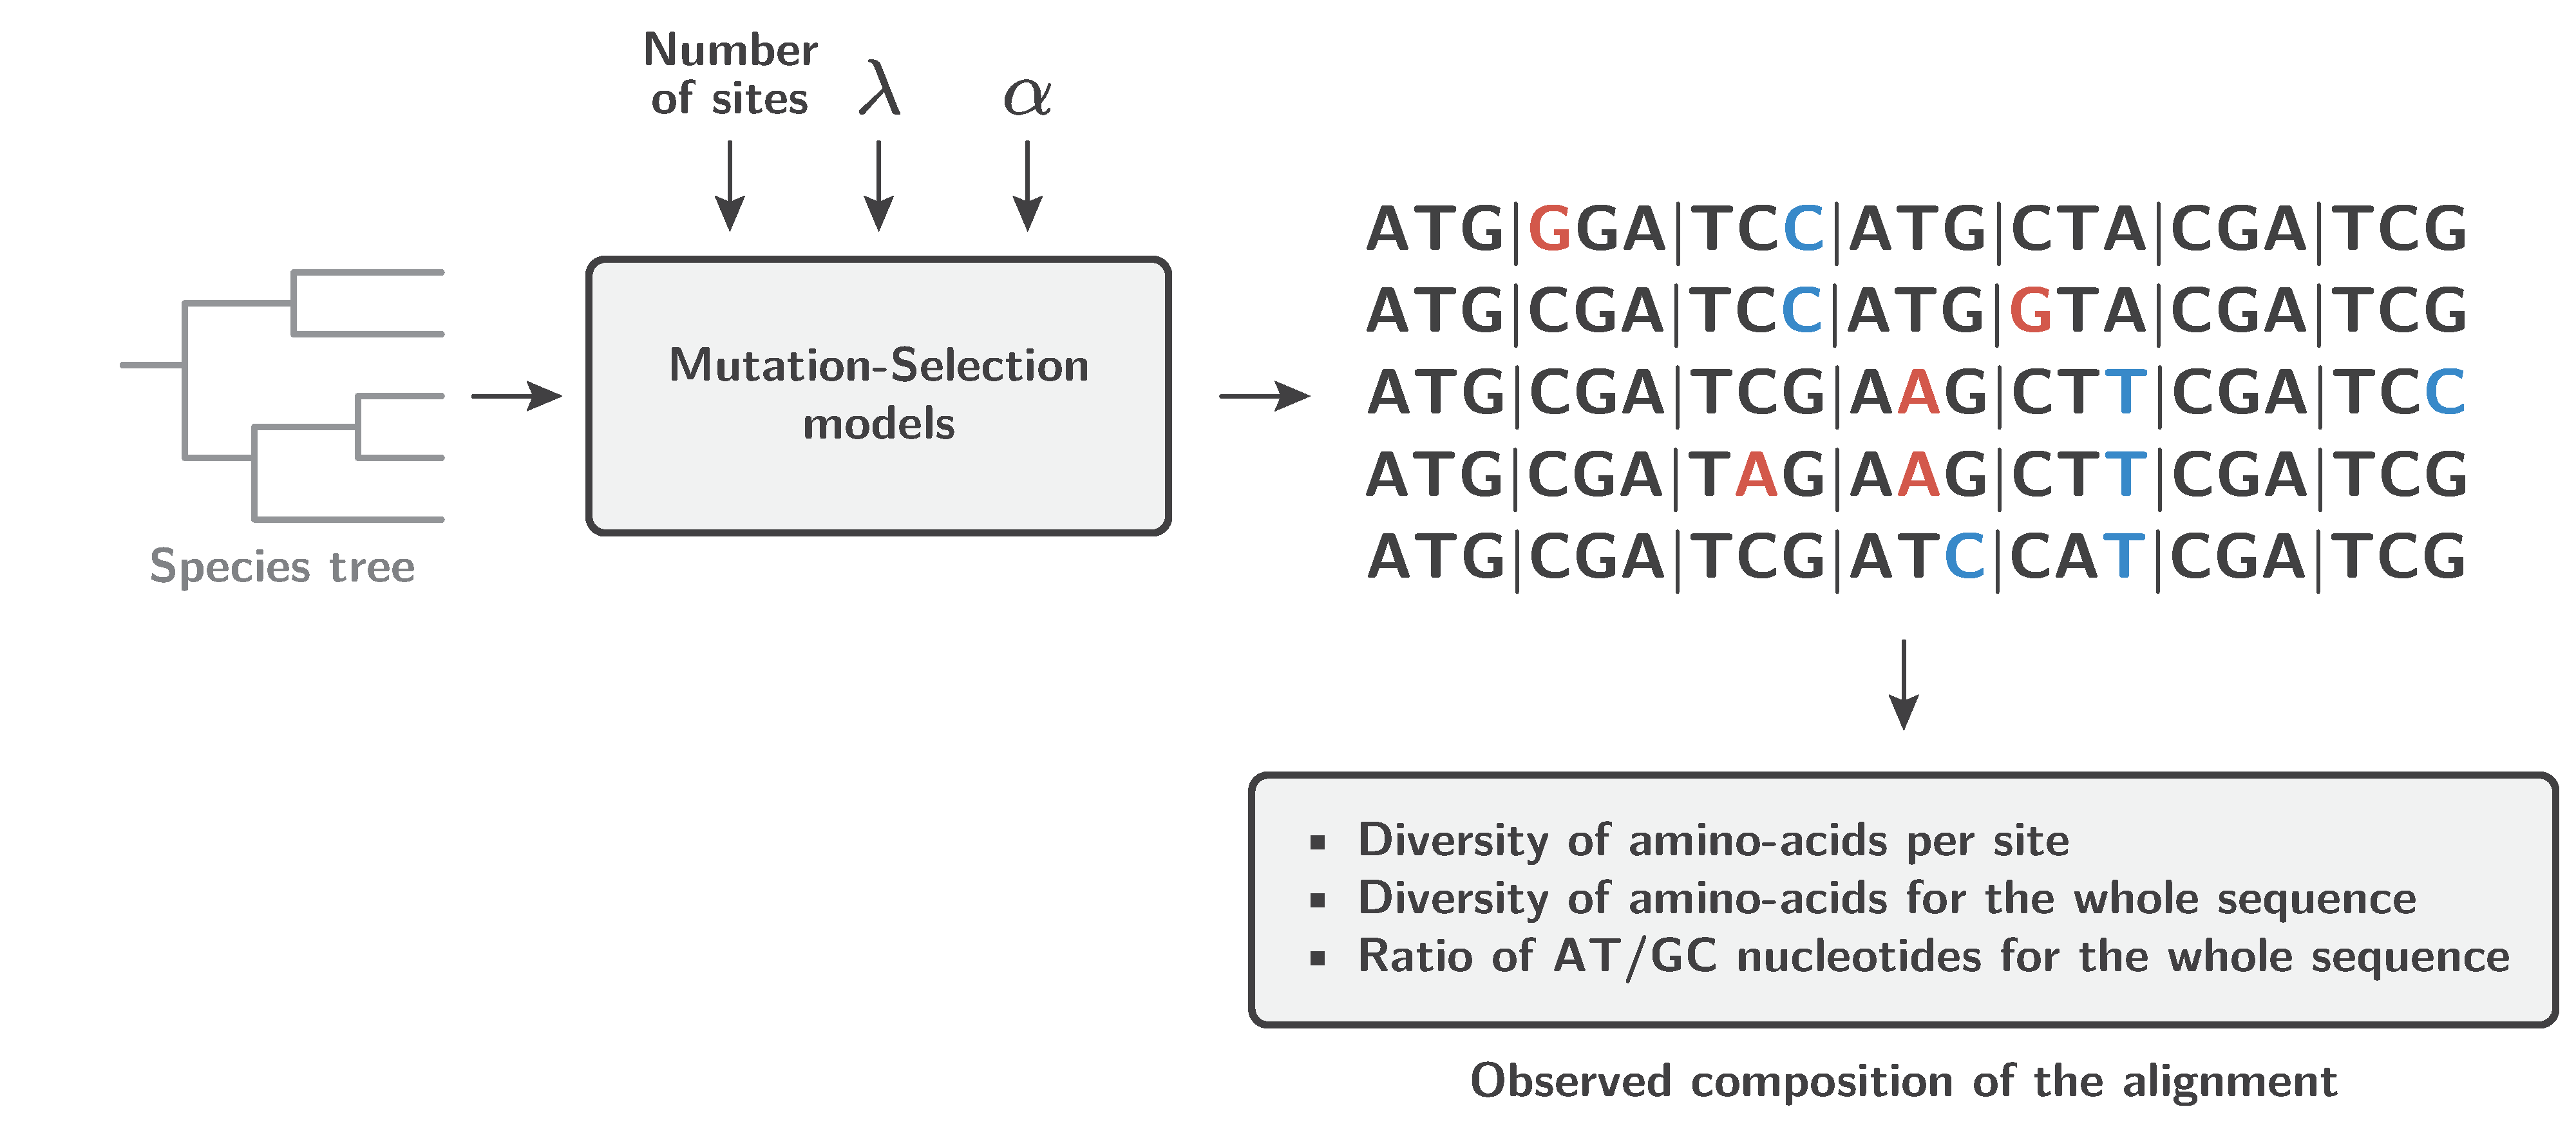
\includegraphics[width=\textwidth] {figures/mut-bias-simulations}
	\end{center}
	\caption[Simulations and analysis]{Simulations and analysis. We can observe composition of the alignment as function of the mutation and selection parameters.}
\end{figure}

\subsection{AT/GC as a function of the mutation-selection model}
The codon substitution process, at site $k$, which takes into account mutation and selection, is a function of $\lambda$ and $F^{(k)}$. Moreover this process has stationary distribution $\pi^{(k)}$. From this equilibrium frequency of codons, we define $\mathrm{AT_{obs}}^{(k)}(\lambda, F^{(k)})$ as the observed stationary distribution of weak nucleotides at site $k$:
\begin{align}
\mathrm{AT_{obs}}^{(k)}(\lambda, F^{(k)})
& =\frac{1}{3} \sum_{x \in \SetCodon} \Pi_x^{(k)} w_x , \ \textrm{by definition},\\
& =\frac{A^{(k)}}{3} \sum_{x \in \SetCodon} \lambda^{w_x} \e^{F_X^{(k)}} w_x , \ \textrm{from eq.} \ \ref{codonStationarity}.
\label{atPctSite}
\end{align}
As noted in \ref{sec:mutBias}, the mutational process leads to $(\pi_A+\pi_T)/(\pi_C+\pi_G) = \lambda$. Similarly, we denote the observed ratio of weak over strong nucleotide frequency, at site $k$, as $\lambda_{\mathrm{obs}}^{(k)} (\lambda, F^{(k)})$:
\begin{align}
\lambda_{\mathrm{obs}}^{(k)} (\lambda, F^{(k)})
& =\dfrac{\mathrm{AT_{obs}}^{(k)}(\lambda, F^{(k)})}{1 - \mathrm{AT_{obs}}^{(k)}(\lambda, F^{(k)}) }, \ \textrm{by definition},\\
& =\dfrac{ \sum_{x \in \SetCodon} \lambda^{w_x} \e^{F_X^{(k)}} w_x}{\sum_{x \in \SetCodon} \lambda^{w_x} \e^{F_X^{(k)}} (3 - w_x )}, \ \textrm{from eq.} \ \ref{atPctSite}.
\end{align}
At the sequence level, $\mathrm{AT_{obs}}(\lambda, \bm{F})$ is the observed stationary distribution of weak nucleotides:
\begin{align}
\mathrm{AT_{obs}}(\lambda, \bm{F})
& =\frac{1}{n}\sum_{k=1}^{n} \mathrm{AT_{obs}}^{(k)}(\lambda, F^{(k)}), \ \textrm{by definition}, \\
& =\frac{1}{3n}\sum_{k=1}^{n} \sum_{x \in \SetCodon} A^{(k)} \lambda^{w_x} \e^{F_X^{(k)}} w_x , \ \textrm{from eq.} \ \ref{atPctSite}.
\label{atPctSeq}
\end{align}
Similarly, we denote the observed ratio of weak over strong nucleotide frequency, for the whole sequence, as $\lambda_{\mathrm{obs}} (\lambda, \bm{F})$
\begin{align}
\lambda_{\mathrm{obs}} (\lambda, \bm{F})
& = \frac{\mathrm{AT_{obs}}(\lambda, \bm{F})}{ 1 - \mathrm{AT_{obs}}(\lambda, \bm{F}) }, \ \textrm{by definition},\\
& =\dfrac{ \sum_{k=1}^{n}  A^{(k)} \sum_{x \in \SetCodon} \lambda^{w_x} \e^{F_X^{(k)}} w_x}{ \sum_{k=1}^{n} A^{(k)} \sum_{x \in \SetCodon} \lambda^{w_x} \e^{F_X^{(k)}} (3 - w_x )}, \ \textrm{from eq.} \ \ref{atPctSeq}.
\end{align}
We then consider amino-acids propensities $S$ (exponential of fitnesses) as a multivariate continuous random variable. More specifically $S$ follow a Dirichlet distribution with concentration parameter $\alpha$.
\begin{equation}
S \sim \mathrm{Dirichlet}(\alpha, 20).
\end{equation}
Under a Dirichlet distribution of amino-acids propensities, the expected observed stationary distribution of weak nucleotides $\operatorname{E} [\mathrm{AT_{obs}}(\lambda, S)]$ is:
\begin{align}
\operatorname{E} [\mathrm{AT_{obs}}(\lambda, S)]
& =\int_{C(s)} \mathrm{AT_{obs}}(\lambda, s) p(s) \der s, \ \textrm{by defintion}, \\
& =\frac{1}{3} \int_{C(s)} A(\lambda, s) \sum_{x \in \SetCodon} 
\lambda^{w_x} s_X w_x p(s) \der s, \ \textrm{from eq.} \ \ref{atPctSite}, \\
& =\frac{1}{3} \int_{ C(s)} A(\lambda, s) \sum_{x \in \SetCodon}  \lambda^{w_x} s_X w_x {\frac {\Gamma (20 \alpha)}{\Gamma (\alpha )^{20}}} \prod_{Y \in \SetAa} s_Y^{\alpha-1} \der s, \\
& ={\frac {\Gamma (20 \alpha)}{3\Gamma (\alpha )^{20}}} \sum_{x \in \SetCodon} \lambda^{w_x} w_x  \int_{ C(s)} A(\lambda, s) s_X \prod_{Y \in \SetAa} s_Y^{\alpha-1} \der s, \\
& ={\frac {\Gamma (20 \alpha)}{3\Gamma (\alpha )^{20}}} \sum_{x \in \SetCodon} \lambda^{w_x} w_x \int_{ C(s)} s_X \dfrac{\prod_{Y \in \SetAa} s_Y^{\alpha-1}}{\sum_{y \in \SetCodon} \lambda^{w_y} s_Y} \der s, \\
& ={\frac {\Gamma (20 \alpha)}{3\Gamma (\alpha )^{20}}} \sum_{x \in \SetCodon} \lambda^{w_x} w_x \Phi_X(\lambda, \alpha),\\
&  \textrm{where} \  \Phi_X(\lambda, \alpha) = \int_{ C(s)} s_X \dfrac{\prod_{Y \in \SetAa} s_Y^{\alpha}}{\sum_{y \in \SetCodon} \lambda^{w_y} s_Y}\der s.
\label{atPctSeqExpected}
\end{align}
Similarly, the observed ratio of weak over strong nucleotide frequency, for the whole sequence, as $\operatorname{E} [\lambda_{\mathrm{obs}}(\lambda, S)]$: 
\begin{align}
\operatorname{E} [\lambda_{\mathrm{obs}}(\lambda, S)]
& =\frac{\operatorname{E} [\mathrm{AT_{obs}}(\lambda, S)]}{ 1 - \operatorname{E} [\mathrm{AT_{obs}}(\lambda, S)] }, \ \textrm{by definition},\\
& =\frac{\sum_{x \in \SetCodon} \lambda^{w_x} w_x \Phi_X(\lambda, \alpha)}{\sum_{x \in \SetCodon} \lambda^{w_x} (3 - w_x) \Phi_X(\lambda, \alpha)}, \ \textrm{from eq.} \ \ref{atPctSeqExpected}.
\label{atgcPctSeqExpected}
\end{align}
For a large sequence ($ n \gg 1 $), $\lambda_{\mathrm{obs}} (\lambda, \bm{F})$ converges to $\operatorname{E} [\lambda_{\mathrm{obs}}(\lambda, S)]$:
\begin{align}
\lambda_{\mathrm{obs}} (\lambda, \bm{F})
& \simeq \operatorname{E} [\lambda_{\mathrm{obs}}(\lambda, S)],\\
& =\frac{\sum_{x \in \SetCodon} \lambda^{w_x} w_x \Phi_X(\lambda, \alpha)}{\sum_{x \in \SetCodon} \lambda^{w_x} (3 - w_x) \Phi_X(\lambda, \alpha)}, \ \textrm{from eq.} \ \ref{atgcPctSeqExpected}.
\end{align}

\begin{figure}[thbp]
	\begin{center}
		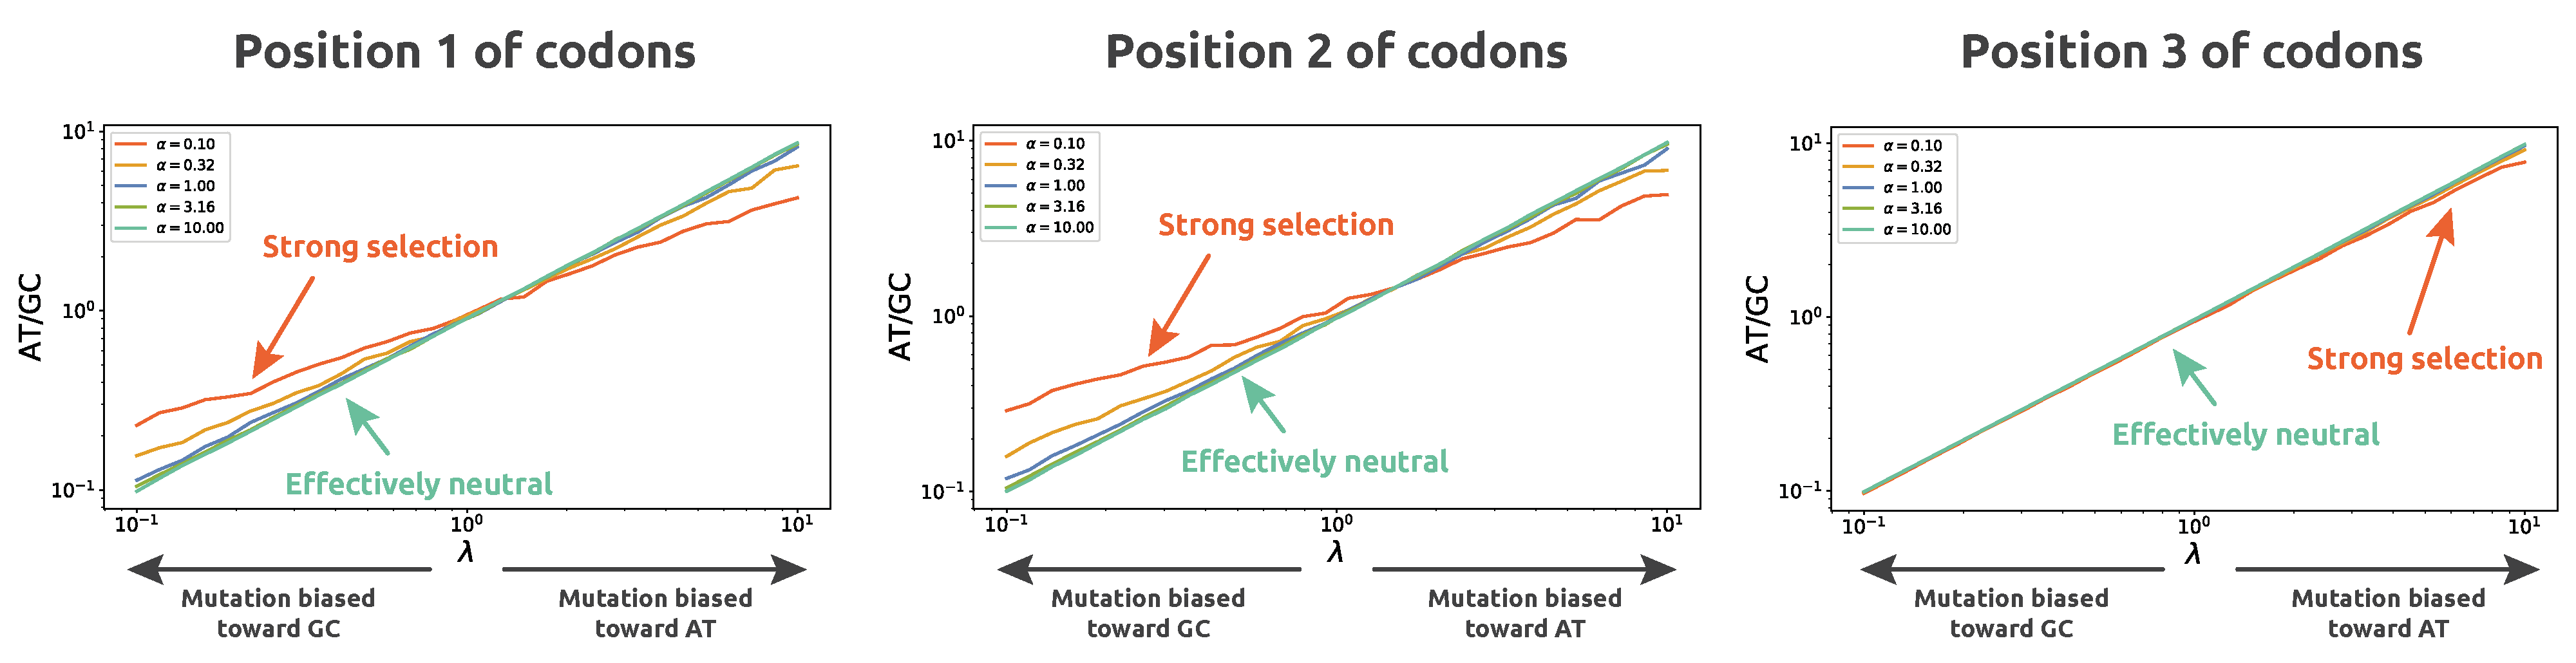
\includegraphics[width=\textwidth] {figures/mut-bias-AT-GC-obs}
	\end{center}
	\caption[AT/GC composition of the alignment]{AT/GC composition of the alignment. Observed AT/GC at the third codon position matches the mutational bias. Selection is balancing the mutational bias.}
\end{figure}

\subsection{Diversity of codons as a function of the mutation-selection model}

The evolutionary variability of an amino acid site in a protein family is an important indicator of the selective constraints that the site experiences. This variability is usually quantified either through the sequence entropy \citep{Goldstein2017}

Our analysis highlights how important it is to distinguish between amino acid frequencies averaged over a large class of sites with similar property (such as RSA) and amino acid frequencies at individual sites. In both cases, frequencies are Boltzmann distributed, and thus it is easy to mistake one for the other. However, the properties of these two distributions are very different. For example, in yeast, at sites with RSA close to 0.2 nearly all amino acids occur at comparable frequencies. Yet at any given site, only a small number ofamino acids are actually permissible. Evolutionary rate, which measures the rate at which mutations at individual sites arise and go to fixation, is governed by the amino acid distribution of individual sites, not the average distribution over a broad class of sites. \citep{Ramsey2011}

The codon substitution process, at site $k$, which takes into account mutation and selection, is a function of $\lambda$ and $F^{(k)}$. Moreover this process has stationary distribution $\pi^{(k)}$. From this equilibrium frequency of codons, we can compute the effective number of codon, mathematically this correspond to the diversity of the distribution $D^{(k)}$, at site $k$:
\begin{align}
D^{(k)}(\lambda, F^{(k)})
& =\e^{ - \sum_{x \in \SetCodon}  \Pi_x^{(k)} \ln ( \Pi_x^{(k)} )}, \ \textrm{by definition},\\
& =\e^{ - \sum_{x \in \SetCodon}  \Pi_x^{(k)} \ln \left( A^{(k)} \lambda^{w_x} \e^{F_X^{(k)}} \right)}, \ \textrm{from eq.} \ \ref{codonStationarity},\\
& =\e^{ - \sum_{x \in \SetCodon}  \Pi_x^{(k)} \left[ \ln ( A^{(k)} )+ \ln( \lambda^{w_x} ) + \ln (\e^{F_X^{(k)}}) \right] }\\
& =\e^{ - \ln ( A^{(k)} ) \sum_{x \in \SetCodon}  \Pi_x^{(k)} } \e^{ -  \ln (\lambda) \sum_{x \in \SetCodon}  \Pi_x^{(k)} w_x }\e^{ - \sum_{x \in \SetCodon}  \Pi_x^{(k)} F_X^{(k)}  } \\
& =\frac{1}{A^{(k)}} \e^{ -  \ln (\lambda) \sum_{x \in \SetCodon}  \Pi_x^{(k)} w_x }\e^{ - \sum_{x \in \SetCodon}  \Pi_x^{(k)} F_X^{(k)}  }
\label{entropy}
\end{align}

\begin{figure}[thbp]
	\begin{center}
		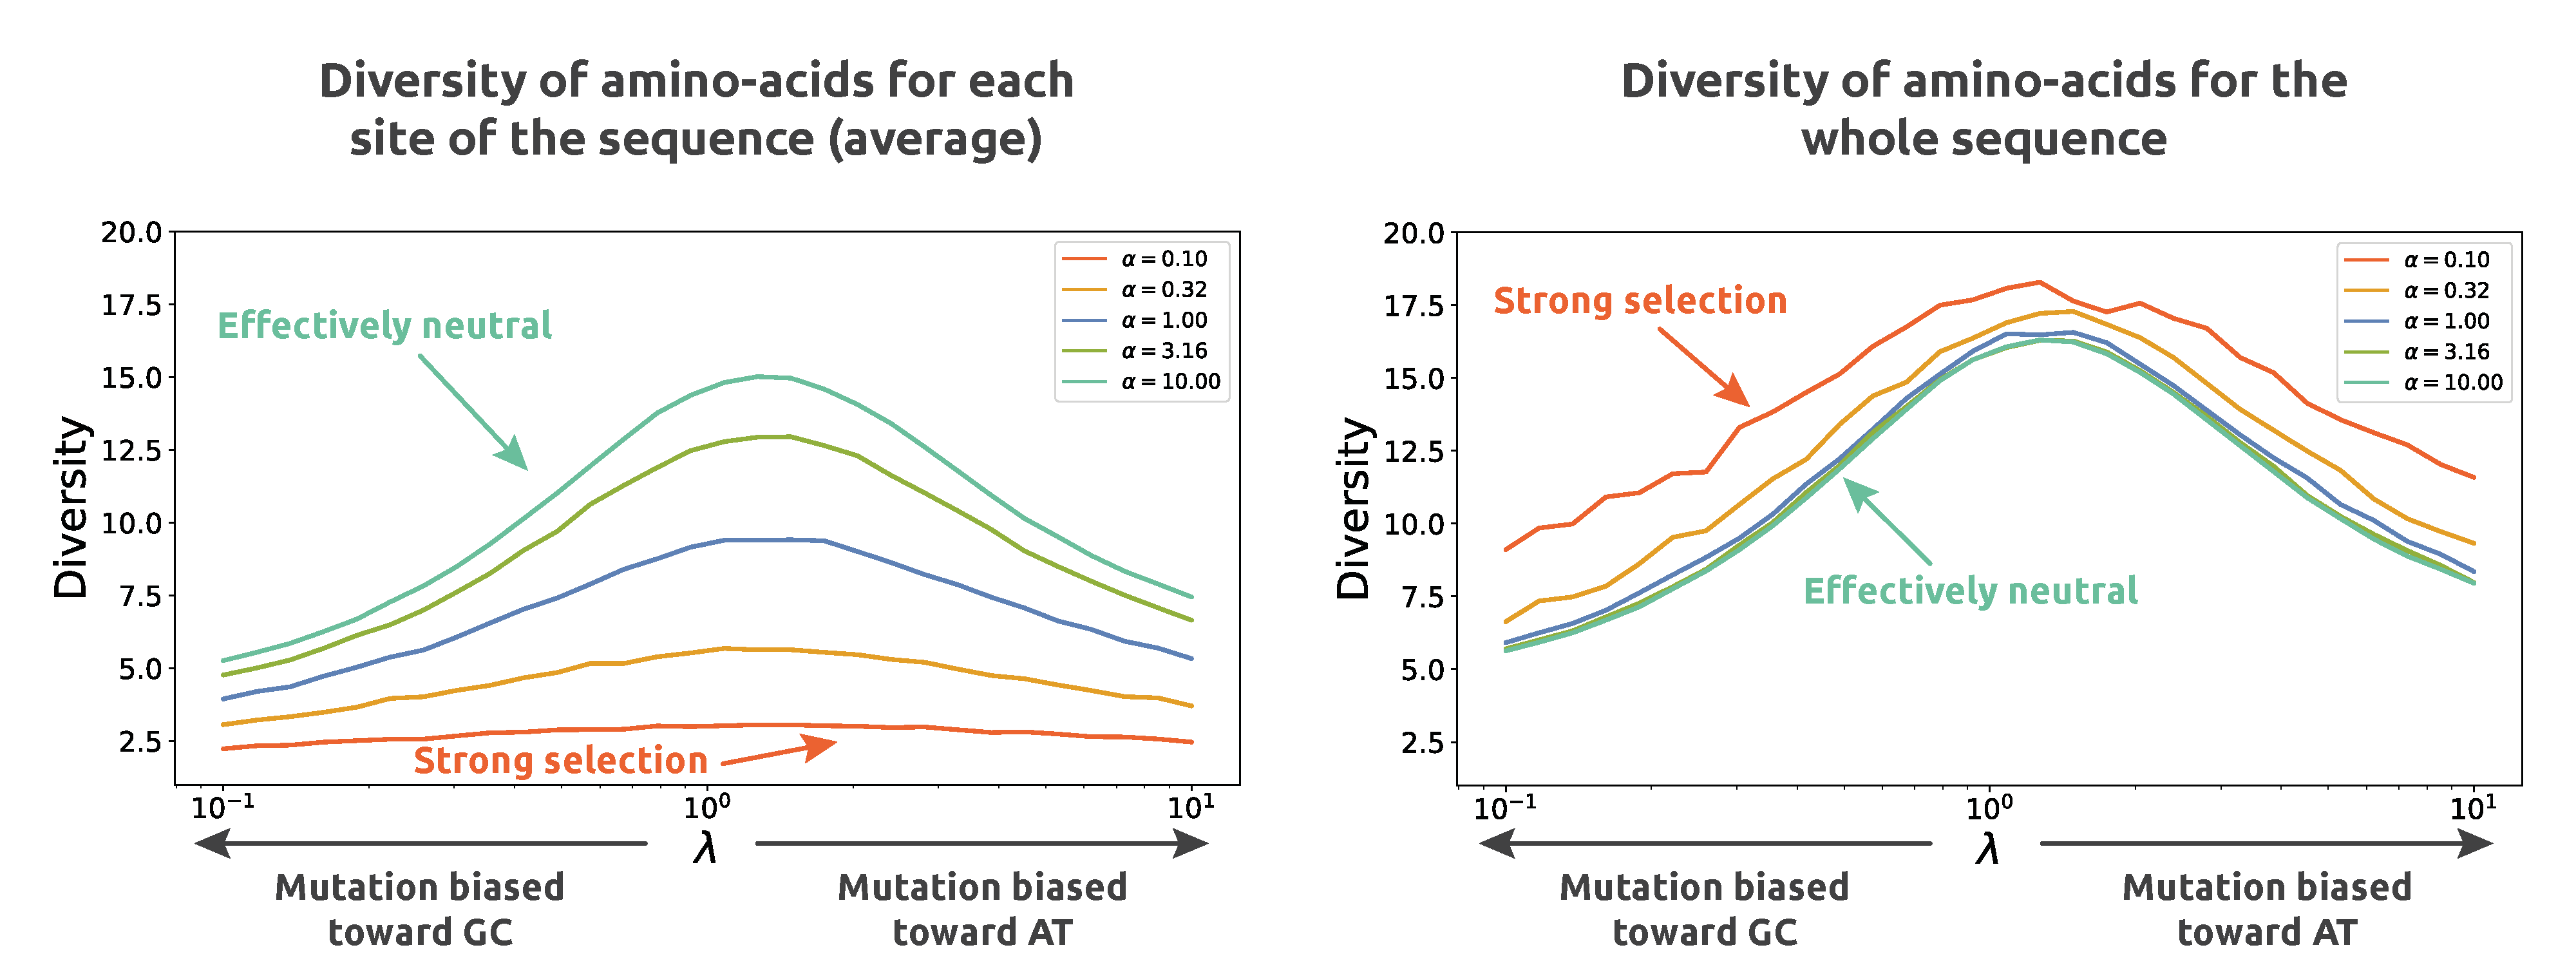
\includegraphics[width=\textwidth] {figures/mut-bias-diversity-aa}
	\end{center}
	\caption[Diversity of amino-acids]{Diversity of amino-acids. Sequence-diversity is higher than site-diversity. Diversity decreases with mutational bias.	Site-diversity decreases with selection. Sequence-diversity increase with selection.}
\end{figure}

\subsection{dN/dS as a function of the mutation-selection model}
The substitution rate (e.g., Grishin, Wolf \& Koonin, 2000). These two measures of evolutionary variability are considered to be essentially equivalent \citep{Halpern1998}, though they are differently influenced by the mutational process \citep{Santos2018}

The codon substitution process, at site $k$, which takes into account mutation and selection, is a function of $\lambda$ and $F^{(k)}$. Moreover this process has stationary distribution $\pi^{(k)}$. From this equilibrium frequency of codons, we define $L_{\NonSyn}^{(k)}(\lambda, F^{(k)})$ as the non-synonymous substitution flow, at site $k$:
\begin{align}
L_{\NonSyn}^{(k)}(\lambda, F^{(k)})
& =  \sum_{x \in \SetCodon} \sum_{y \in \NxNonSyn} \Pi_x^{(k)} Q_{x, y}^{(k)}, \ \textrm{by definition},\\
& =\sum_{x \in \SetCodon} \sum_{y \in \NxNonSyn} A^{(k)} \lambda^{w_x} \e^{F_X^{(k)}} U_{x, y} \dfrac{F_Y^{(k)} - F_X^{(k)}}{1 - \e^{F_X^{(k)} - F_Y^{(k)}}}, \ \textrm{from eq.}\ \ref{codonSubRates} \ \text{and} \ \ref{codonStationarity},\\
& =A^{(k)} \sum_{x \in \SetCodon} \lambda^{w_x} \sum_{y \in \NxNonSyn}  U_{x, y} \dfrac{F_Y^{(k)} - F_X^{(k)}}{\e^{-F_X^{(k)}} - \e^{ - F_Y^{(k)}}}.
\label{subFlowNonSyn}
\end{align}
Moreover, we define $K_{\NonSyn}^{(k)}(\lambda, F^{(k)})$ as the non-synonymous mutation flow, at site $k$:
\begin{align}
K_{\NonSyn}^{(k)}(\lambda, F^{(k)})
& =  \sum_{x \in \SetCodon} \sum_{y \in \NxNonSyn} \Pi_x^{(k)} U_{x, y}, \ \textrm{by definition},\\
& = A^{(k)}  \sum_{x \in \SetCodon} \lambda^{w_x} \sum_{y \in \NxNonSyn} \e^{F_X^{(k)}} U_{x, y}, \ \textrm{from eq.}\ \ref{codonSubRates} \ \text{and} \ \ref{codonStationarity}.
\label{mutFlowNonSyn}
\end{align}
We also define the mutation and substitution synonymous as $K_{\Syn}^{(k)}(\lambda, F^{(k)})$ and $L_{\Syn}^{(k)}(\lambda, F^{(k)})$ respectively:
\begin{align}
L_{\Syn}^{(k)}(\lambda, F^{(k)})
& =  \sum_{x \in \SetCodon} \sum_{y \in \NxSyn} \Pi_x^{(k)} Q_{x, y}^{(k)}, \ \textrm{by definition},\\
& =\sum_{x \in \SetCodon} \sum_{y \in \NxSyn} A^{(k)} \lambda^{w_x} \e^{F_X^{(k)}} U_{x, y}, \ \textrm{from eq.}\ \ref{codonSubRates} \ \text{and} \ \ref{codonStationarity}, \\
& =K_{\Syn}^{(k)}(\lambda, F^{(k)})
\label{subFlowSyn}
\end{align}
Following Spielman and Wilke \citep{Spielman2015}, the rate of non-synonymous to synonymous substitution is thus :
\begin{align}
\omega^{(k)}(\lambda, F^{(k)})
& =\dfrac{L_{\NonSyn}^{(k)}(\lambda, F^{(k)})}{K_{\NonSyn}^{(k)}(\lambda, F^{(k)})}  \left( \dfrac{L_{\Syn}^{(k)}(\lambda, F^{(k)})}{K_{\Syn}^{(k)}(\lambda, F^{(k)})}  \right)^{-1}, \\
& =\dfrac{L_{\NonSyn}^{(k)}(\lambda, F^{(k)})}{K_{\NonSyn}^{(k)}(\lambda, F^{(k)})}, \ \textrm{from eq.}\ \ref{subFlowSyn} \\
& =\dfrac{ \sum_{x \in \SetCodon} \lambda^{w_x} \sum_{y \in \NxNonSyn}  U_{x, y} \dfrac{F_Y^{(k)} - F_X^{(k)}}{\e^{ - F_Y^{(k)}} -  \e^{- F_X^{(k)}} } }{ \sum_{x \in \SetCodon}  \lambda^{w_x} \sum_{y \in \NxNonSyn} U_{x, y} \e^{F_X^{(k)}} }, \ \textrm{from eq.}\ \ref{subFlowNonSyn} \ \text{and} \ \ref{mutFlowNonSyn}.
\label{omegaSite}
\end{align}
The non-synonymous over synonymous rate for the whole sequence is then given by:
\begin{align}
\omega(\lambda, \bm{F})
& =\dfrac{\sum_{k=1}^{n} L_{\NonSyn}^{(k)}(\lambda, F^{(k)})}{\sum_{k=1}^{n}K_{\NonSyn}^{(k)}(\lambda, F^{(k)})}  \left( \dfrac{\sum_{k=1}^{n}L_{\Syn}^{(k)}(\lambda, F^{(k)})}{\sum_{k=1}^{n}K_{\Syn}^{(k)}(\lambda, F^{(k)})}  \right)^{-1}, \\
& =\dfrac{\sum_{k=1}^{n} L_{\NonSyn}^{(k)}(\lambda, F^{(k)})}{\sum_{k=1}^{n}K_{\NonSyn}^{(k)}(\lambda, F^{(k)})}, \ \textrm{from eq.}\ \ref{subFlowSyn} \\
& =\dfrac{ \sum_{k=1}^{n} \sum_{x \in \SetCodon} \lambda^{w_x} \sum_{y \in \NxNonSyn}  U_{x, y} \dfrac{F_Y^{(k)} - F_X^{(k)}}{\e^{ - F_Y^{(k)}} -  \e^{- F_X^{(k)}} } }{ \sum_{k=1}^{n} \sum_{x \in \SetCodon}  \lambda^{w_x}  \sum_{y \in \NxNonSyn} U_{x, y} \e^{F_X^{(k)}}}, \ \textrm{from eq.}\ \ref{subFlowNonSyn} \ \text{and} \ \ref{mutFlowNonSyn}. \\
& =\dfrac{ \sum_{x \in \SetCodon} \lambda^{w_x} \sum_{y \in \NxNonSyn}  U_{x, y}  \sum_{k=1}^{n} \dfrac{F_Y^{(k)} - F_X^{(k)}}{\e^{ - F_Y^{(k)}} -  \e^{- F_X^{(k)}} } }{  \sum_{x \in \SetCodon}  \lambda^{w_x}  \sum_{y \in \NxNonSyn} U_{x, y}  \sum_{k=1}^{n} \e^{F_X^{(k)}}}.
\label{omegaSeq}
\end{align}
We then consider amino-acids propensities $S$ (exponential of fitnesses) as a multivariate continuous random variable. More specifically $S$ follow a Dirichlet distribution with concentration parameter $\alpha$.
\begin{equation}
S \sim \mathrm{Dirichlet}(\alpha, 20).
\end{equation}
Under a Dirichlet distribution of amino-acids propensities, the expected non-synonymous substitution flow $\operatorname{E} [L_{\NonSyn}(\lambda, S)]$ :
\begin{align}
\operatorname{E} [L_{\NonSyn}(\lambda, S)]
& =\int_{C(s)} L_{\NonSyn}(\lambda, s) p(s) \der s, \ \textrm{by defintion}, \\
& =\int_{C(s)} A(\lambda, s) \sum_{x \in \SetCodon} \lambda^{w_x} \sum_{y \in \NxNonSyn} U_{x, y} s_X s_Y\dfrac{\ln(s_Y)-\ln(s_X)}{s_Y - s_Y} p(s) \der s , \ \textrm{from eq.}\ \ref{subFlowNonSyn}, \\
& =\int_{C(s)} A(\lambda, s) \sum_{x \in \SetCodon} \lambda^{w_x} \sum_{y \in \NxNonSyn} U_{x, y} s_X s_Y\dfrac{\ln(s_Y)-\ln(s_X)}{s_Y - s_Y} {\frac {\Gamma (20 \alpha)}{\Gamma (\alpha )^{20}}} \prod_{X \in \SetAa} s_X^{\alpha-1} \der s,\\
& ={\frac {\Gamma (20 \alpha)}{\Gamma (\alpha )^{20}}} \sum_{x \in \SetCodon} \lambda^{w_x} \sum_{y \in \NxNonSyn} U_{x, y} \int_{C(s)} s_Y\dfrac{\ln(s_Y)-\ln(s_X)}{s_Y - s_Y} \dfrac{\prod_{X \in \SetAa} s_X^{\alpha}}{\sum_{y \in \SetCodon} \lambda^{w_y} s_Y} \der s.\\
& ={\frac {\Gamma (20 \alpha)}{\Gamma (\alpha )^{20}}} \sum_{x \in \SetCodon} \lambda^{w_x} \sum_{y \in \NxNonSyn} U_{x, y} \Psi(\lambda, \alpha), \\
& \textrm{where} \ \Psi(\lambda, \alpha) = \int_{C(s)} s_Y\dfrac{\ln(s_Y)-\ln(s_X)}{s_Y - s_Y} \dfrac{\prod_{X \in \SetAa} s_X^{\alpha}}{\sum_{y \in \SetCodon} \lambda^{w_y} s_Y} \der s.
\end{align}
Moreover, the expected non-synonymous mutation flow $\operatorname{E} [K_{\NonSyn}(\lambda, S)]$ is:
\begin{align}
\operatorname{E} [K_{\NonSyn}(\lambda, S)]
& =  \int_{C(s)} K_{\NonSyn}(\lambda, s) p(s) \der s, \ \textrm{by defintion}, \\
& =\int_{C(s)} A(\lambda, s) \sum_{x \in \SetCodon} \lambda^{w_x} \sum_{y \in \NxNonSyn} s_X U_{x, y} p(s) \der s , \ \textrm{from eq.}\ \ref{mutFlowNonSyn}, \\
& =\int_{C(s)} A(\lambda, s) \sum_{x \in \SetCodon} \lambda^{w_x} \sum_{y \in \NxNonSyn} s_X U_{x, y}{\frac {\Gamma (20 \alpha)}{\Gamma (\alpha )^{20}}} \prod_{X \in \SetAa} s_X^{\alpha-1} \der s,\\
& =\frac{\Gamma (20 \alpha)}{\Gamma (\alpha )^{20}} \sum_{x \in \SetCodon} \lambda^{w_x} \sum_{y \in \NxNonSyn} U_{x, y} \int_{C(s)} \dfrac{\prod_{X \in \SetAa} s_X^{\alpha}}{\sum_{y \in \SetCodon} \lambda^{w_y} s_Y}\der s,\\
& =\frac{\Gamma (20 \alpha)}{\Gamma (\alpha )^{20}} \sum_{x \in \SetCodon} \lambda^{w_x} \sum_{y \in \NxNonSyn} U_{x, y} \Phi(\lambda, \alpha).\\
\end{align}
The expected non-synonymous over synonymous rate, $\operatorname{E} [\omega(\lambda, S)]$ , is then given by:
\begin{align}
\operatorname{E} [\omega(\lambda, S)]
& =  \dfrac{\operatorname{E} [L_{\NonSyn}(\lambda, S)]}{\operatorname{E} [K_{\NonSyn}(\lambda, S)]} \\
& =\dfrac{\sum_{x \in \SetCodon} \lambda^{w_x} \sum_{y \in \NxNonSyn} U_{x, y} \Psi(\lambda, \alpha)}{\sum_{x \in \SetCodon} \lambda^{w_x} \sum_{y \in \NxNonSyn} U_{x, y} \Phi(\lambda, \alpha)}.
\label{omegaExpected}
\end{align}
For a large sequence ($ n \gg 1 $), $\omega (\lambda, \bm{F})$ converges to $\operatorname{E} [\omega(\lambda, S)]$:
\begin{align}
\omega (\lambda, \bm{F})
& \simeq \operatorname{E} [\omega(\lambda, S)],\\
& =\dfrac{\sum_{x \in \SetCodon} \lambda^{w_x} \sum_{y \in \NxNonSyn} U_{x, y} \Psi(\lambda, \alpha)}{\sum_{x \in \SetCodon} \lambda^{w_x} \sum_{y \in \NxNonSyn} U_{x, y} \Phi(\lambda, \alpha)}, \ \textrm{from eq.} \ \ref{omegaExpected}.
\end{align}

\begin{figure}[thbp]
	\begin{center}
		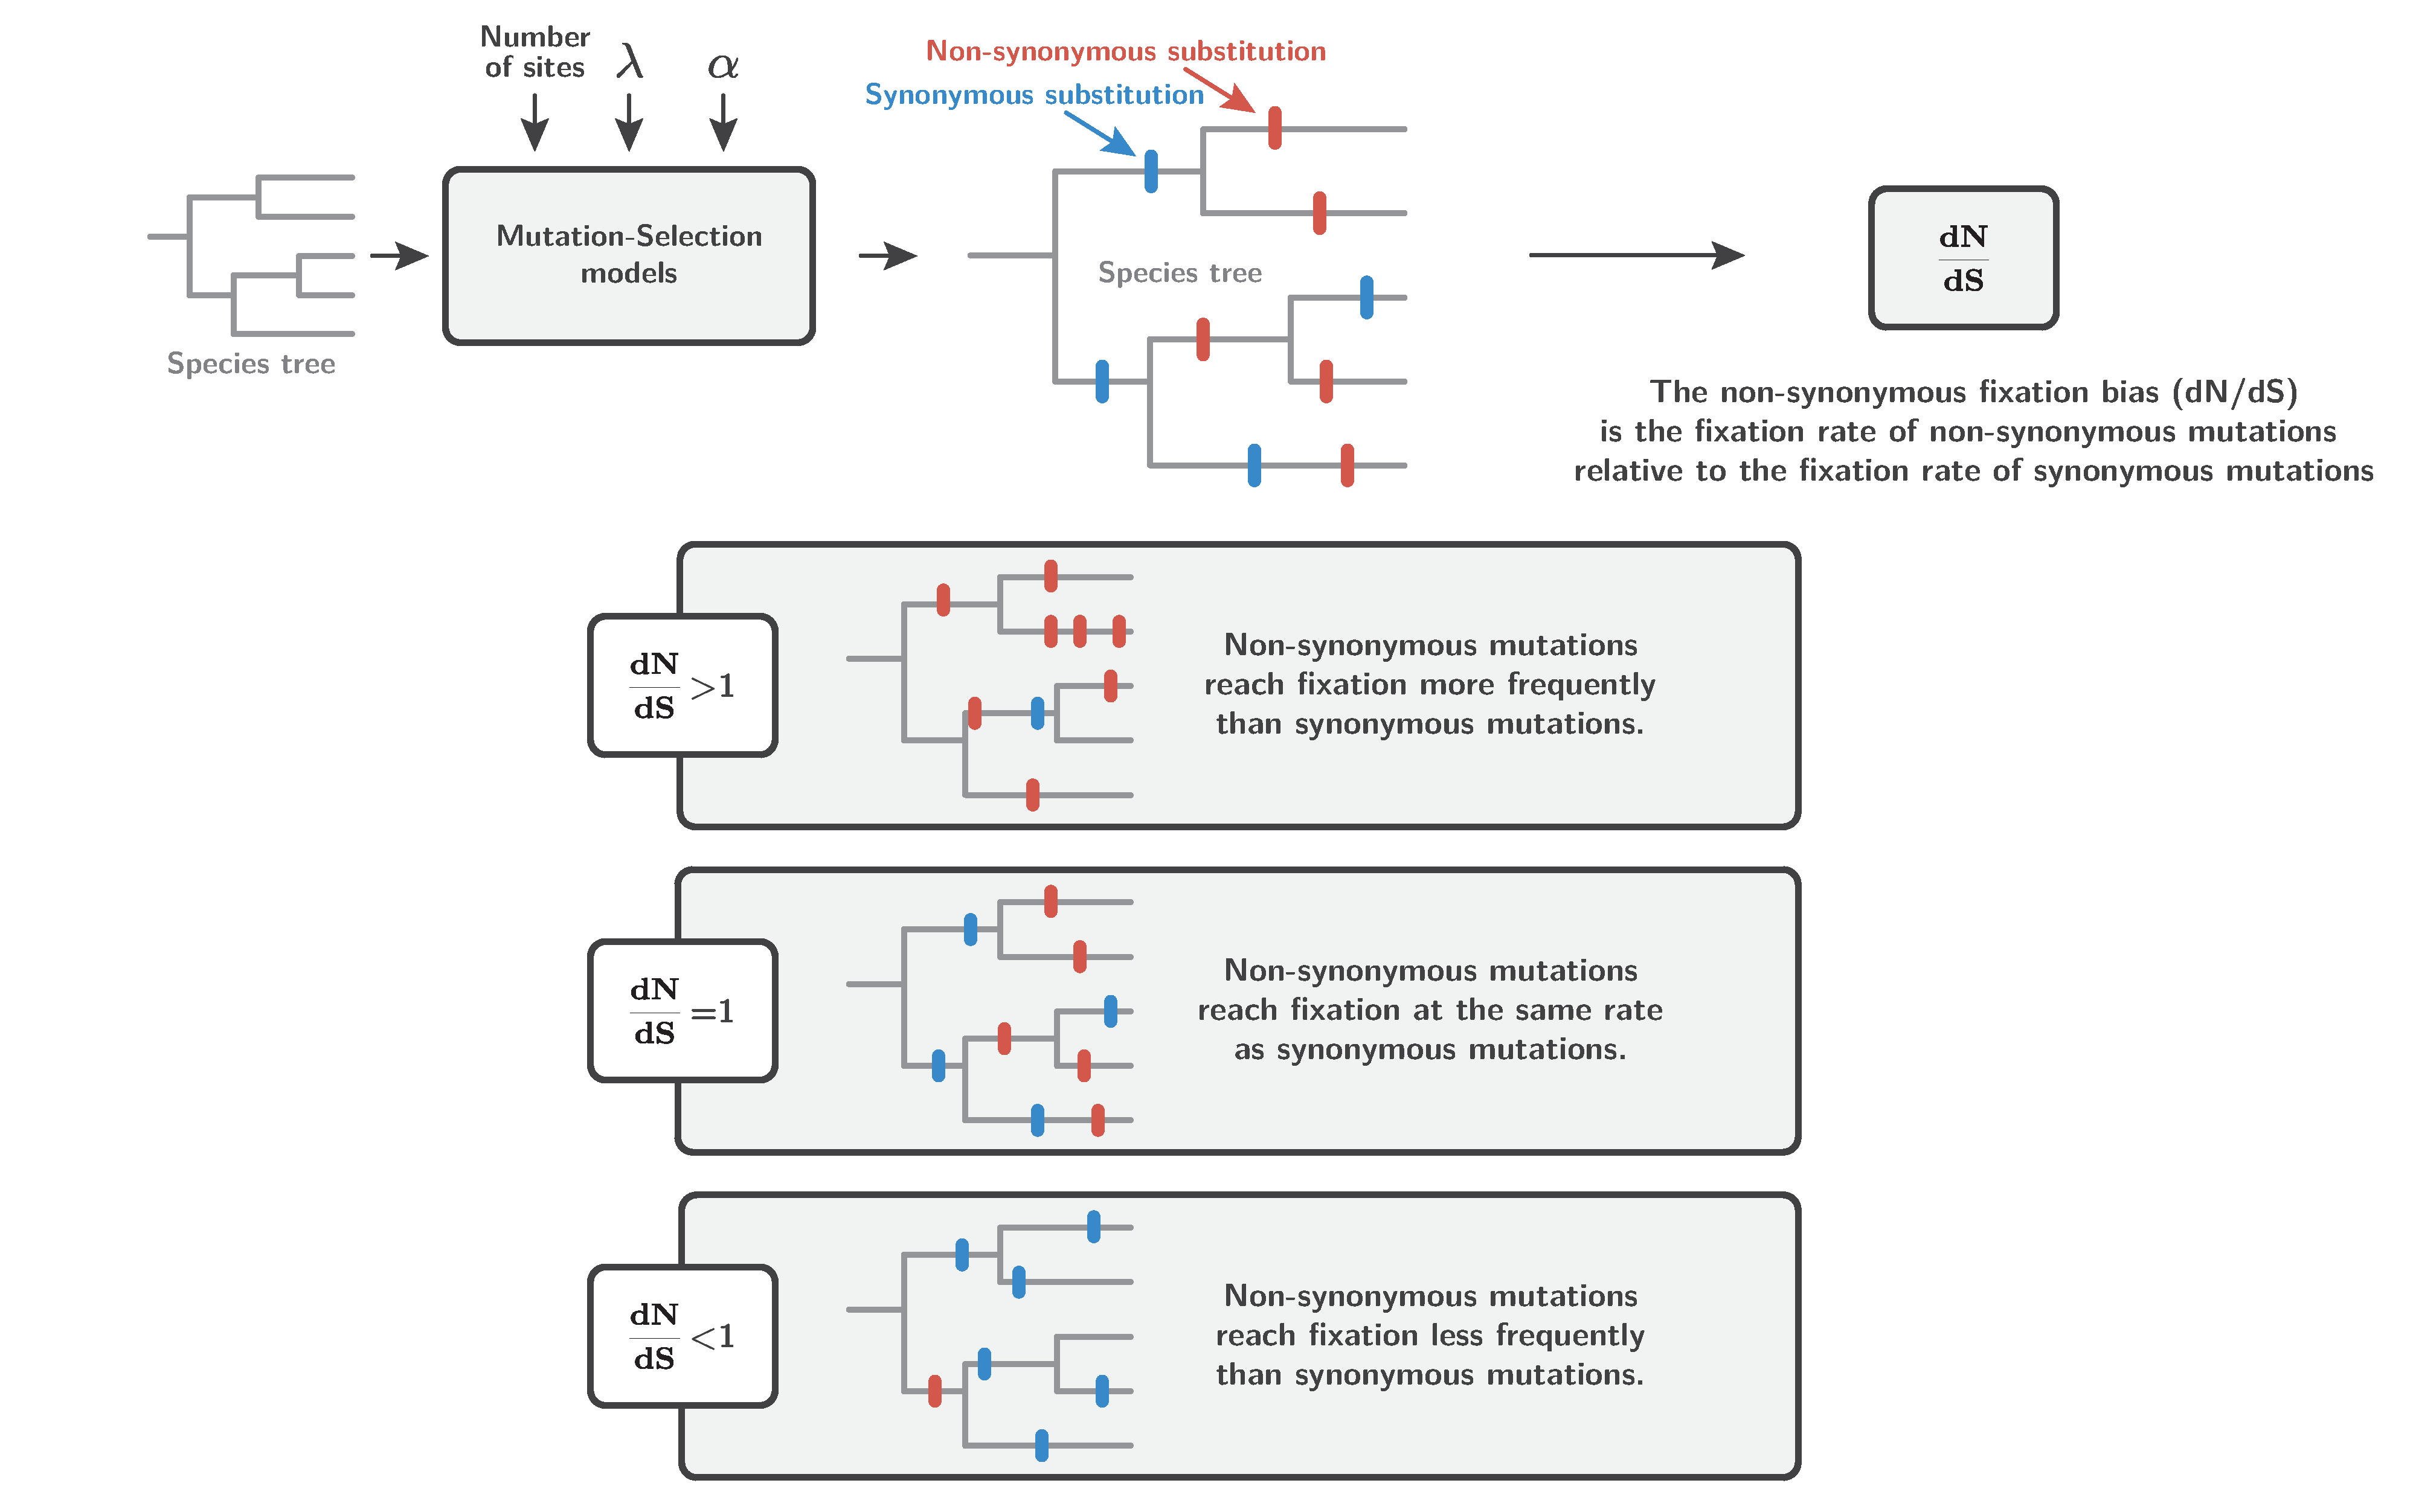
\includegraphics[width=\textwidth] {figures/mut-bias-definitions}
	\end{center}
	\caption[Definition of $\omega$]{Definition of $\omega$.}
\end{figure}

\begin{figure}[thbp]
	\begin{center}
		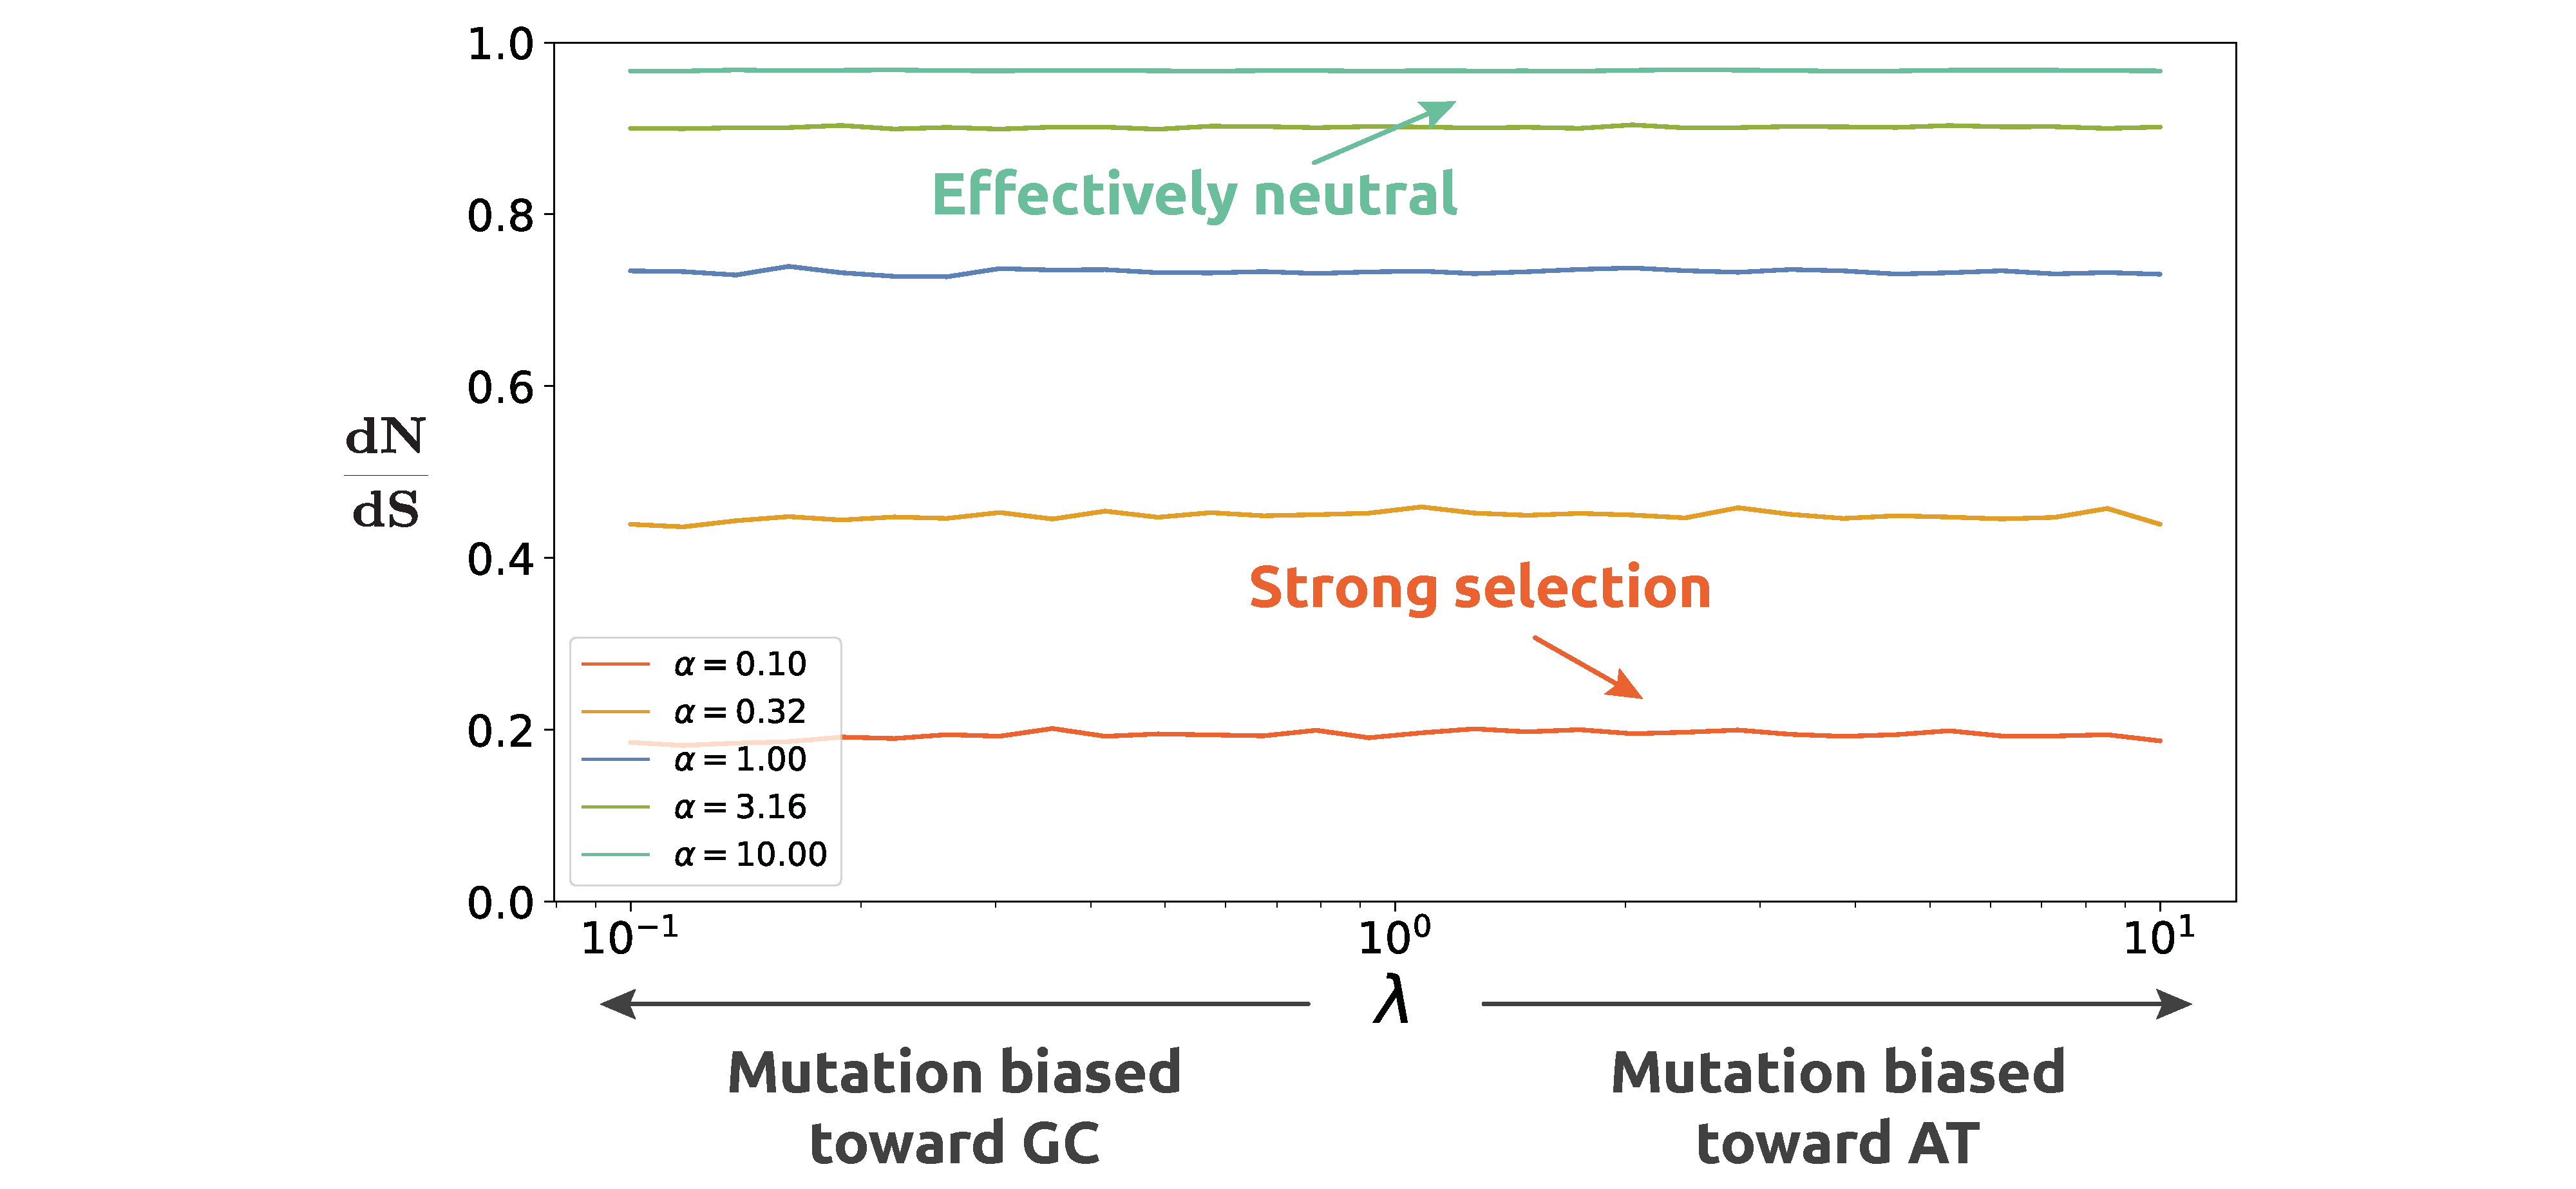
\includegraphics[width=\textwidth] {figures/mut-bias-omega}
	\end{center}
	\caption[$\omega$ as a function of the parameters]{$\omega$ as a function of the parameters. Non-synonymous fixation bias is always lower than. Non-synonymous fixation bias decrease with the strength of selection. Non-synonymous fixation bias is unaffected by mutational bias.}
\end{figure}

\begin{figure}[thbp]
	\begin{center}
		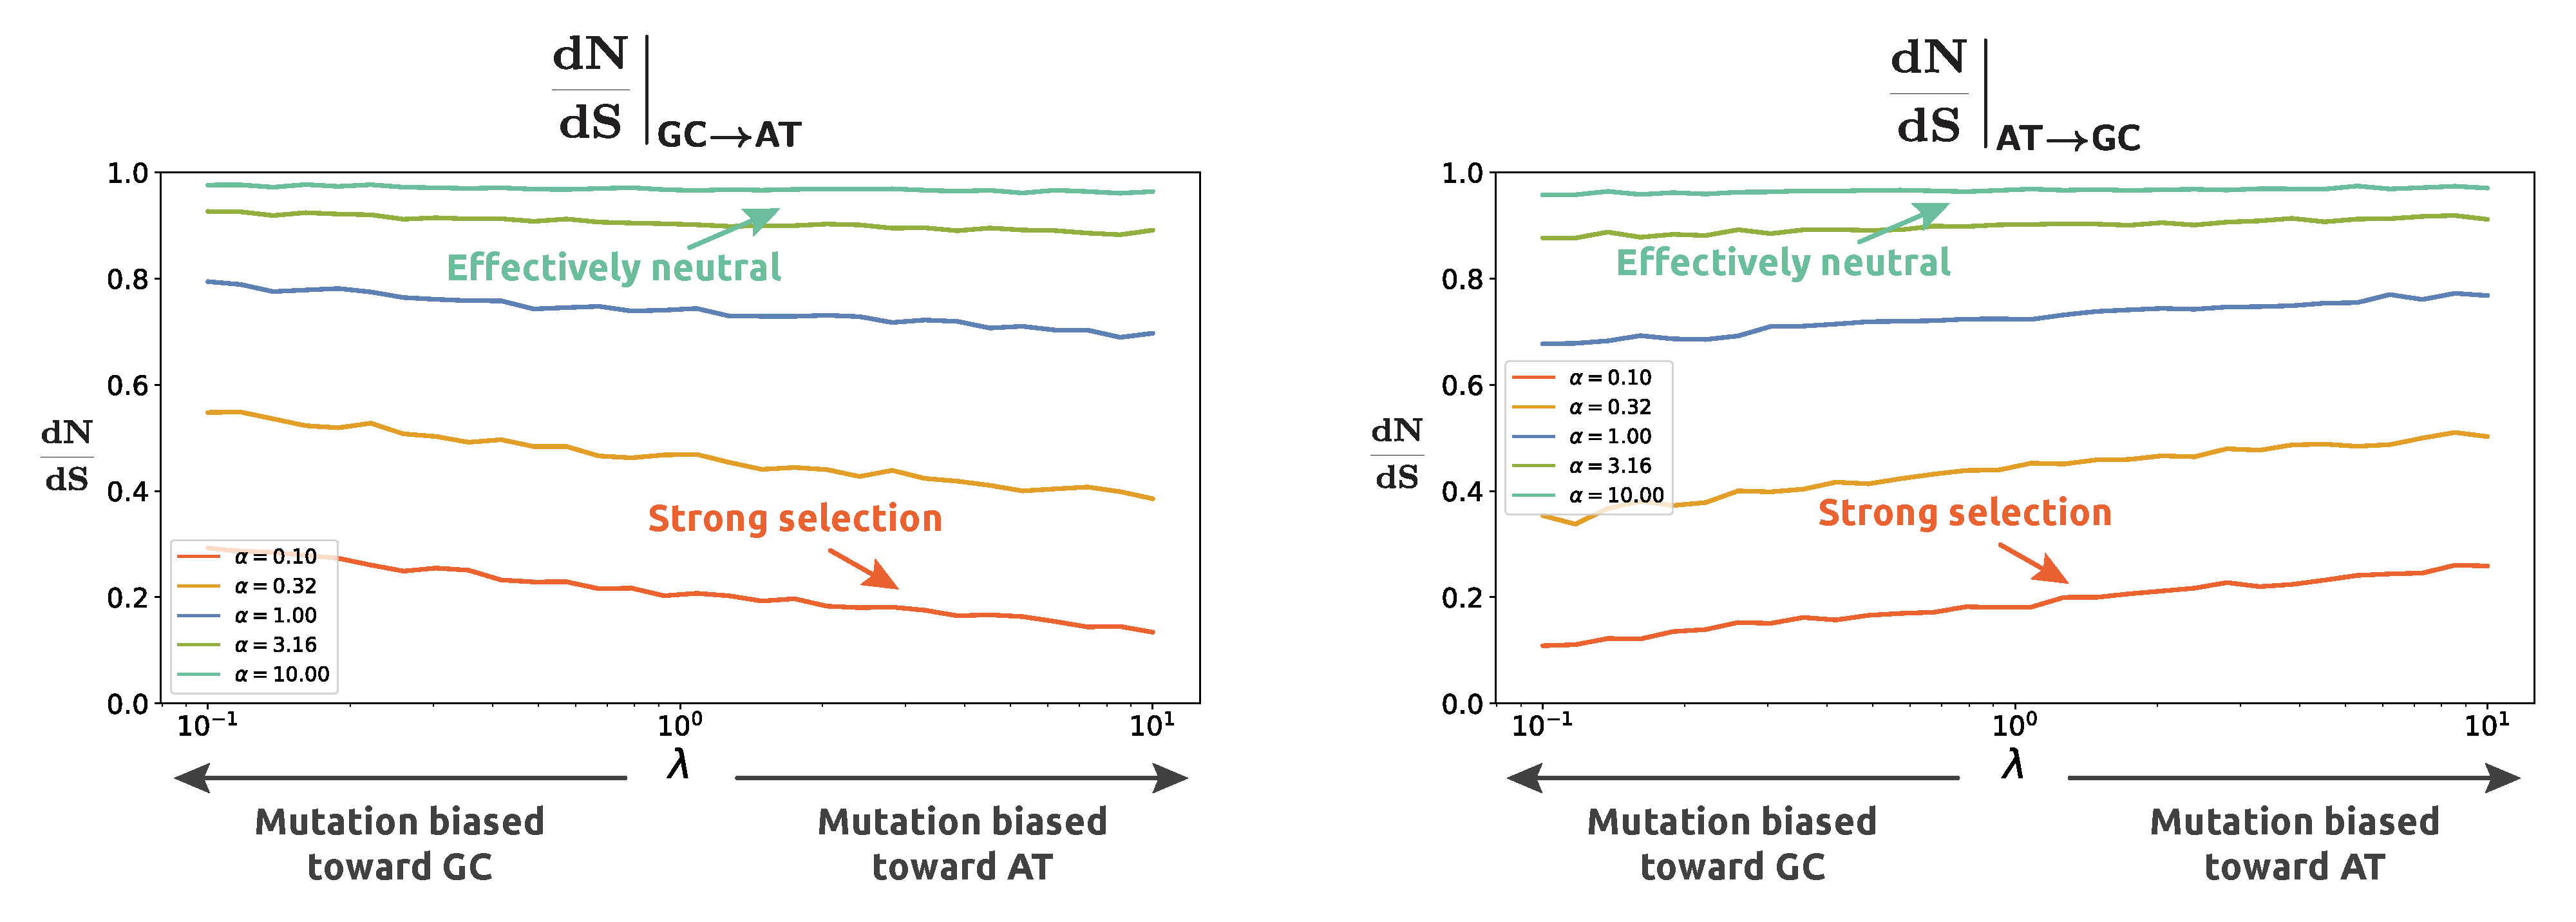
\includegraphics[width=\textwidth, page=1] {figures/mut-bias-omega-WS-SW}
	\end{center}
	\caption[Fixation bias of non-synonymous mutations]{Fixation bias of non-synonymous mutations. Mutation biased from GC to AT leads to a fixation bias in the opposite direction. More generally, mutation bias leads to balancing fixation bias. This is confounding factor with gBGC.}
\end{figure}

\section{Parametric inference}

\begin{figure}[thbp]
	\begin{center}
		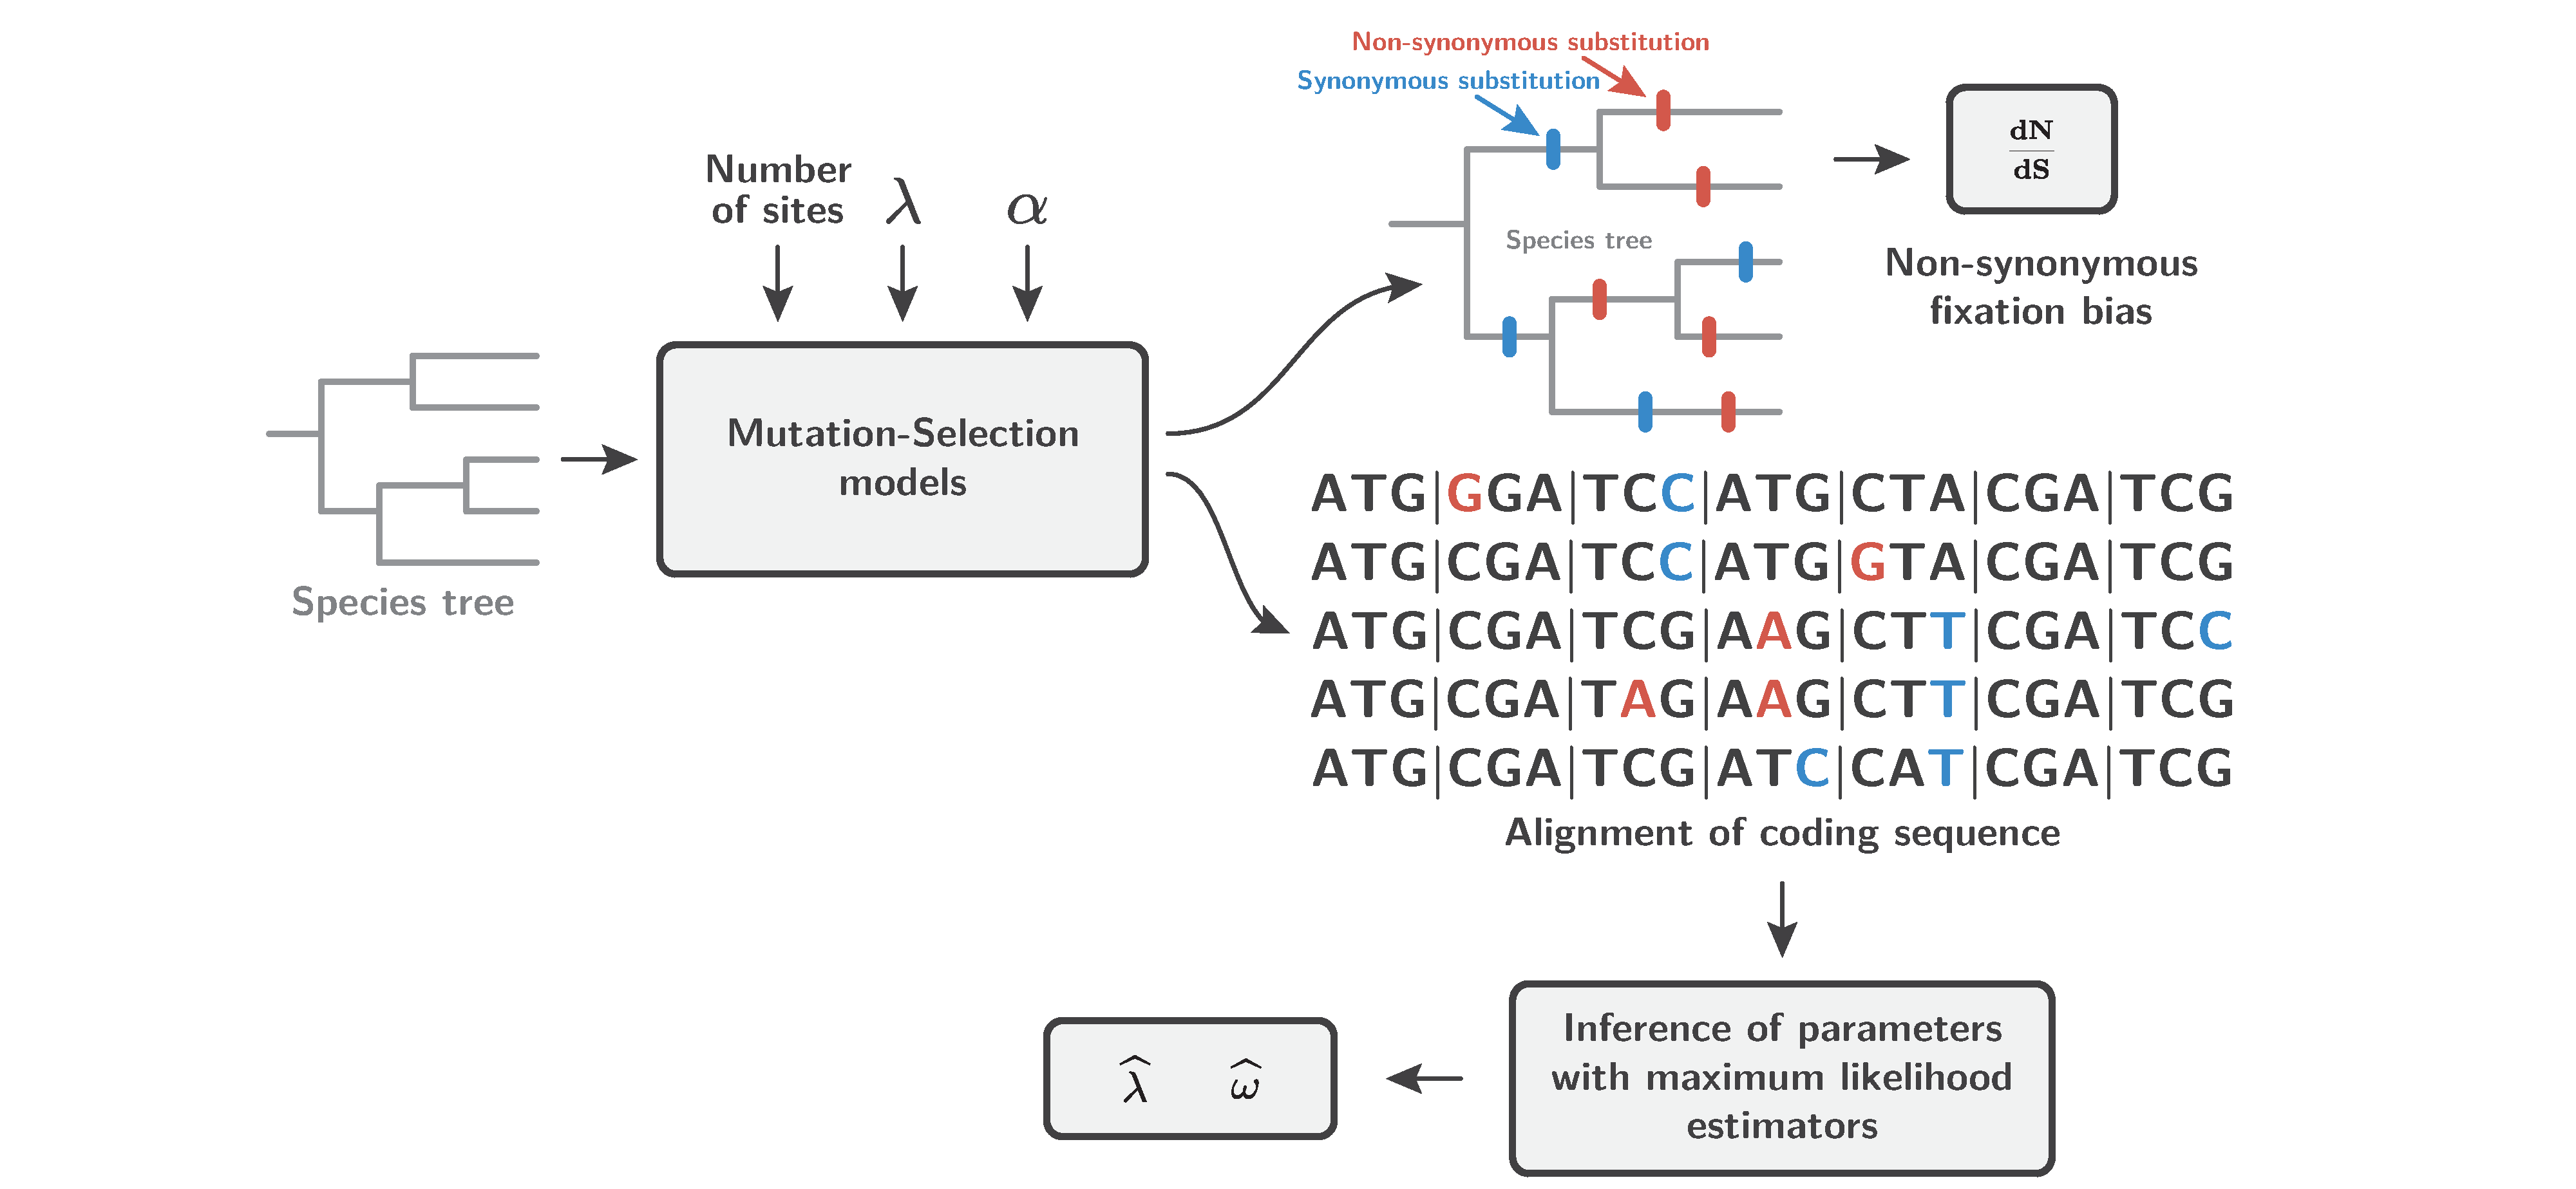
\includegraphics[width=\textwidth] {figures/mut-bias-pipeline}
	\end{center}
	\caption[Inferred value compared to known value]{Inferred value compared to known value.}
\end{figure}

\subsection{Parametric inference with Muse-Gaut model}

\begin{itemize}
	\item ${q_{{\color{RED}{\textbf{ATT}}} \rightarrow {\color{GREEN}\textbf{ATG}}}}$ is the substitution rate from codon ${\color{RED}{\textbf{ATT}}}$ to ${\color{GREEN}\textbf{ATG}}$.
	\item ${\mu_{{\color{RED}\textbf{T}} \rightarrow {\color{GREEN}\textbf{G}}}}$ is the mutation rate from nucleotide ${\color{RED}\textbf{T}}$ to ${\color{GREEN}\textbf{G}}$ 
	\item ${\omega}$ is the non-synonymous fixation bias. 
\end{itemize}
\begin{equation*}
\begin{dcases}
{q_{{\color{RED}{\textbf{ATT}}} \rightarrow {\color{GREEN}\textbf{ATG}}}} = { \omega \mu_{{\color{RED}\textbf{T}} \rightarrow {\color{GREEN}\textbf{G}}} } & \text{since } {\color{RED}{\textbf{ATT}}} \text{ and } {\color{GREEN}\textbf{ATG}} \text{ are non-synonymous} \\
{q_{{\color{RED}{\textbf{ATT}}} \rightarrow {\color{BLUE}\textbf{ATA}}}} = { \mu_{{\color{RED}\textbf{T}} \rightarrow {\color{BLUE}\textbf{A}}}} & \text{since } {\color{RED}{\textbf{ATT}}} \text{ and } {\color{BLUE}\textbf{ATA}} \text{ are synonymous}\\
\end{dcases}
\end{equation*}
From the maximum likelihood estimates of the $4 \times 4$ mutation matrix $\left({\widehat{\mu}} \right)$, we can estimate of the mutational bias toward $\mathrm{AT}$ $\left({\widehat{\lambda}_{\text{MG}}} \right)$. We can also estimate the fixation bias of non-synonymous mutations $\left({\widehat{\omega}_{\text{MG}}} \right)$


\subsection{Inference under projected mutation-selection}
\begin{itemize}
	\item ${\beta_{{\color{RED}{\textbf{Ile}}} \rightarrow {\color{GREEN}{\textbf{Met}}}}}$ is the fixation bias from Isoleucine to Methionine
\end{itemize}
\begin{equation*}
\begin{dcases}
{q_{{\color{RED}{\textbf{ATT}}} \rightarrow {\color{GREEN}\textbf{ATG}}}} = { \beta_{{\color{RED}{\textbf{Ile}}} \rightarrow {\color{GREEN}{\textbf{Met}}}} \mu_{{\color{RED}\textbf{T}} \rightarrow {\color{GREEN}\textbf{G}}}} & \text{since } {\color{RED}{\textbf{ATT}}} \text{ and } {\color{GREEN}\textbf{ATG}} \text{ are non-synonymous} \\
{q_{{\color{RED}{\textbf{ATT}}} \rightarrow {\color{BLUE}\textbf{ATA}}}} = {\mu_{{\color{RED}\textbf{T}} \rightarrow {\color{BLUE}\textbf{A}}} } & \text{since } {\color{RED}{\textbf{ATT}}} \text{ and } {\color{BLUE}\textbf{ATA}} \text{ are synonymous}\\
\end{dcases}
\end{equation*}
From the maximum likelihood estimates of the $4 \times 4$ mutation matrix $\left({\widehat{\mu}} \right)$, we can estimate the mutational bias $\mathrm{AT}$ $\left({\widehat{\lambda}_{\text{MF}}} \right)$. We can also estimate the fixation bias of non-synonymous mutations $\left({\widehat{\omega}_{\text{MF}}} \right)$


\begin{figure}[thbp]
	\begin{center}
		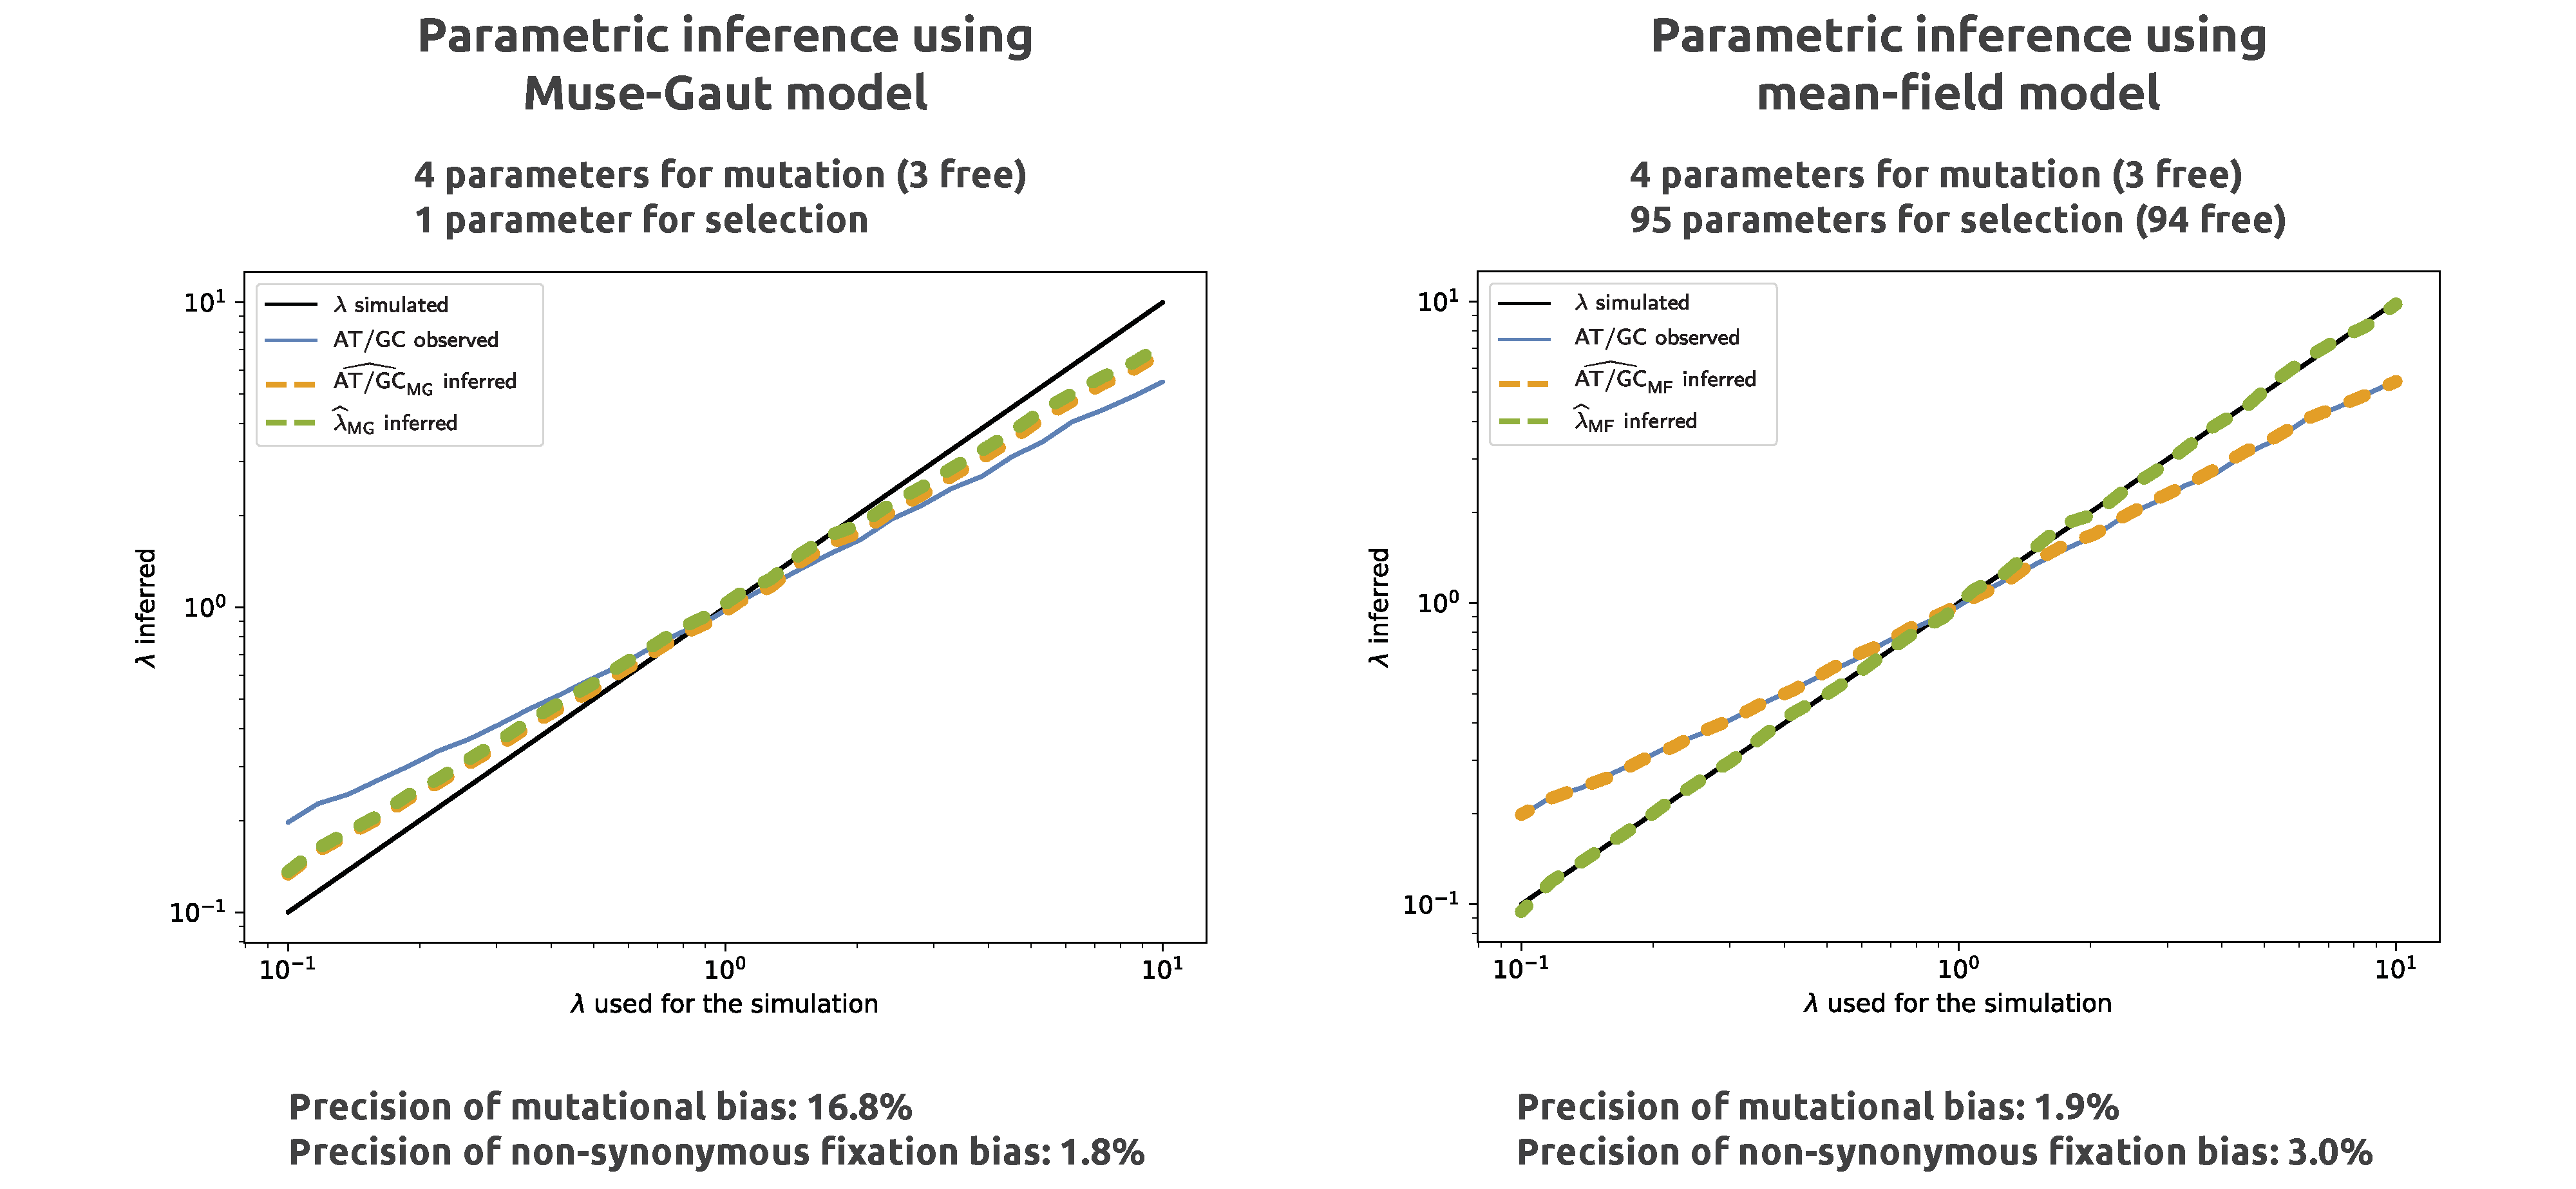
\includegraphics[width=\textwidth] {figures/mut-bias-Simulation-vs-Inference}
	\end{center}
	\caption[Estimation of mutation and fixation bias]{Estimation of mutation and fixation bias. Modeling a single fixation bias leads to skewed estimation of mutation bias. Modeling multiple fixation bias leads to precise estimation of mutation bias. Estimation of fixation bias doesn't depend on the underlying mutation bias.}
\end{figure}

\subsection{Experiment I: Nucleoprotein}
Alignment of 498 amino-acids available for 180 species.
\begin{itemize}
	\item AT/GC of the alignment is 1.15.
	\item Mutational bias $\left({\widehat{\lambda}_{\text{MG}}} \right)$ inferred using Muse-Gaut model is 1.39.
	\item Mutational bias $\left({\widehat{\lambda}_{\text{MF}}} \right)$ inferred using Mean-field model is 1.64.
	\item Fixation bias from AT to GC $\left(\widehat{\omega}_{\textbf{AT} \rightarrow \textbf{GC}}\right)$ inferred using Mean-field model is 0.14.
	\item Fixation bias from GC to AT $\left(\widehat{\omega}_{\textbf{GC} \rightarrow \textbf{AT}}\right)$ inferred using Mean-field model is 0.10.
\end{itemize}
\subsection{Experiment II: Lactamase}
Alignment of 263 amino-acids available for 85 species.
\begin{itemize}
	\item AT/GC of the alignment is 0.79.
	\item Mutational bias $\left({\widehat{\lambda}_{\text{MG}}} \right)$ inferred using Muse-Gaut model is 0.85.
	\item Mutational bias $\left({\widehat{\lambda}_{\text{MF}}} \right)$ inferred using Mean-field model is 0.68.
	\item Fixation bias from AT to GC $\left(\widehat{\omega}_{\textbf{AT} \rightarrow \textbf{GC}}\right)$ inferred using Mean-field model is 0.31.
	\item Fixation bias from GC to AT $\left(\widehat{\omega}_{\textbf{GC} \rightarrow \textbf{AT}}\right)$ inferred using Mean-field model is 0.44.
\end{itemize}

The observed composition of the alignment is the result of the articulation between mutation and selection.
Mutational bias is balanced by a fixation bias (selection) in the opposite direction, potentially a confounding effect with gBGC.
Inference of mutational bias requires to model fixation bias in different direction.
Our mean-field parametric framework is not site-wise, but can be used to untangle mutation and selection, potentially in the presence of fluctuating selection or epistasis.
